% !TeX encoding = UTF-8
% !TeX program = pdflatex
% !BIB program = bibtex

%%% Um einen Artikel auf deutsch zu schreiben, genügt es die Klasse ohne
%%% Parameter zu laden.
\documentclass[]{lni}
\usepackage{microtype}
\usepackage{csquotes}
\usepackage{listings}

\newcommand{\quoteStyle}{alphabetic}

\usepackage[
    backend=biber,		% recommended. Alternative: bibtex
    bibwarn=true,
    bibencoding=utf8,	         % If .bib file is encoded with utf8, otherwise ascii
    sortlocale=de_DE,
    style=\quoteStyle,
]{biblatex}
\usepackage{graphics}
\usepackage{graphicx}

\addbibresource{lni-author-template.bib}

%%% To write an article in English, please use the option ``english'' in order
%%% to get the correct hyphenation patterns and terms.
%%% \documentclass[english]{class}
%%
\begin{document}
%%% Mehrere Autoren werden durch \and voneinander getrennt.
%%% Die Fußnote enthält die Adresse sowie eine E-Mail-Adresse.
%%% Das optionale Argument (sofern angegeben) wird für die Kopfzeile verwendet.
\title[Hybride Applikationen]{Vergleich von Frameworks zur Entwicklung hybrider Applikationen}
%%%\subtitle{Untertitel / Subtitle} % if needed
\author[Jannik Dürr \and Dominic Joas \and Ruben Kalmbach]
{Jannik Dürr\footnote{DHBW Stuttgart Campus Horb, Studiengang Informatik, Florianstraße 15, 72160 Horb am Neckar, Deutschland, \email{i20007@hb.dhbw-stuttgart.de}} \and
Dominic Joas\footnote{DHBW Stuttgart Campus Horb, Studiengang Informatik, Florianstraße 15, 72160 Horb am Neckar, Deutschland, \email{i20015@hb.dhbw-stuttgart.de}} \and
Ruben Kalmbach\footnote{DHBW Stuttgart Campus Horb, Studiengang Informatik, Florianstraße 15, 72160 Horb am Neckar, Deutschland, \email{i20018@hb.dhbw-stuttgart.de}}}
\startpage{1} % Beginn der Seitenzählung für diesen Beitrag / Start page
\editor{Herausgeber et al.} % Names of Editors
\booktitle{Advanced Software Engineering 2022} % Name of book title
\yearofpublication{2022}
%%%\lnidoi{18.18420/provided-by-editor-02} % if known
\maketitle

\begin{abstract}
Hybride Applikationen sind ein moderner Ansatz zur Vereinfachung der Softwareentwicklung. Basierend auf einer gemeinsamen Codebasis wird die Anwendung durch native Wrapper zu verschiedenen Betriebssystemen kompatibel gemacht. Aufgrund der großen Anzahl an Frameworks für die Entwicklung hybrider Applikationen werden in diesem Beitrag verschiedene Frameworks gegenübergestellt. Zunächst werden der Aufbau und die Eigenschaften hybrider Anwendungen beschrieben, sowie Vergleichskriterien und relevante Merkmale hybrider Frameworks zusammengefasst. Dann werden drei Anwendungsgebiete definiert: rechenintensiv, formularlastig und sensorlastig. Die Vergleichskriterien werden in einem paarweisen Vergleich für jedes Anwendungsgebiet separat gewichtet. Anschließend werden die einzelnen Frameworks mithilfe von Literatur und eigenen Untersuchungen betrachtet und anhand der Kriterien bewertet. Durch die Berechnung der Punktzahlen für jedes Framework können Empfehlungen für jedes Anwendungsgebiet gegeben werden.
\end{abstract}
\begin{keywords}
Hybride Applikation \and Hybride Frameworks \and Mobile Applikation \and Native Applikation %Keyword1 \and Keyword2 
\end{keywords}


%%% Beginn des Artikeltexts
\section{Einleitung}
In diesem Kapitel wird eine Einleitung in den Beitrag in Form einer Motivation gegeben. Anschließend werden die verwendeten Methoden erläutert, gefolgt von einem Überblick über das Vorgehen und die Ziele.

\subsection{Motivation}

Applikationen auf mobilen Geräten nehmen im Alltag vieler Menschen eine große Rolle ein. In den App-Stores von Google und Apple stehen mehrere Millionen Apps zur Verfügung, die jeden Bereich des täglichen Lebens abdecken. Bei vielen dieser Apps handelt es sich um native Applikationen, seit einigen Jahren gewinnen jedoch hybride Applikationen ebenfalls immer mehr an Popularität und kommen z.\,B. bei Social-Media-Apps wie Twitter erfolgreich zum Einsatz.

Hybride Applikationen versuchen, die Vorteile von nativen Applikationen und Web-Applikationen zu kombinieren. Native Applikationen sind Anwendungen, die speziell für ein konkretes Betriebssystem entwickelt und optimiert wurden. Web-Applikationen sind hingegen vollständig browserbasiert und unabhängig von konkreten Betriebssystemen, allerdings ist der Zugriff auf die Sensoren des Geräts stark eingeschränkt. Einen guten Kompromiss bilden die bereits angesprochenen hybriden Applikationen, die wie Web-Anwendungen mit Webtechnologien entwickelt werden, allerdings anschließend in native Container, auch Wrapper genannt, verpackt werden. So sind sie kompatibel zu mehreren Betriebssystemen und können dabei auf native Schnittstellen zugreifen. Der Arbeitsaufwand, der bei der Entwicklung von Apps ein zentraler Faktor ist, kann so stark reduziert werden, da die Entwicklung nicht für jedes Betriebssystem separat erfolgen muss. 

Für die Entwicklung von hybriden Applikationen stehen eine Vielzahl an Frameworks zur Verfügung. Abbildung \ref{fig:statistikFrameworks} stellt diesbezüglich dar, welche hybriden Frameworks weltweit von Entwicklern bevorzugt verwendet werden. Allerdings ist es für Entwickler, die sich nicht intensiv mit der Entwicklung hybrider Applikationen beschäftigt haben, oft schwierig zu entscheiden, welches Framework für bestimmte Anwendungsfälle verwendet werden sollte. Daher werden in dieser Arbeit die wichtigsten hybriden Frameworks genauer betrachtet und anhand definierter Kriterien miteinander verglichen. So können Empfehlungen abgegeben werden, welches Framework abhängig von den Anforderungen eingesetzt werden sollte. \\

\begin{figure}[h]
	\centering
	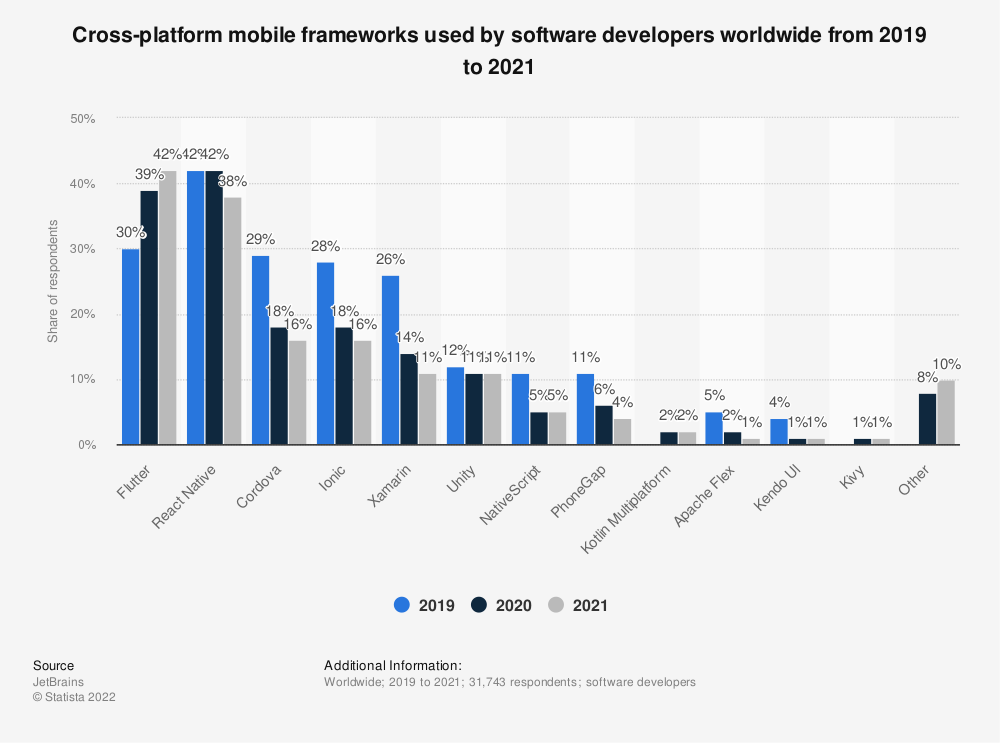
\includegraphics[width=\linewidth]{images/statistik_frameworks.png}
	\caption{Umfrage, welche hybriden Frameworks von Entwicklern verwendet werden \cite{Statista.21.10.2022}}
	\label{fig:statistikFrameworks}
\end{figure}


\subsection{Methoden}
Folgende Methoden werden neben der Literaturarbeit verwendet:
\begin{itemize}
	\item \textbf{Paarweiser Vergleich} \\
		Durch einen paarweisen Vergleich werden die Vergleichskriterien systematisch paarweise gegenübergestellt und so ermittelt, welches der Kriterien wichtiger ist bzw. ob sie gleich wichtig sind. Aus der numerischen Interpretation der Gegenübergestellungen ergeben sich die Rangfolge und die relative Gewichtung der Vergleichskriterien.
	\item \textbf{Prototyping} \\
		Durch die Entwicklung von Prototypen mit möglichst identischem Funktionsumfang werden Erfahrungen mit den Frameworks gesammelt und der Entwicklungsaufwand bewertet.
	\item \textbf{Benchmarking} \\
		Durch die Durchführung eines Software-Benchmarks mit identischen Algorithmen werden Ausführungszeiten und CPU-Auslastung der Prototypen ermittelt.
\end{itemize}

\subsection{Vorgehen und Ziele}
Das Ziel des Beitrags ist der Vergleich von Frameworks zur Entwicklung hybrider Applikationen. Zu diesem Zweck werden hybride Applikationen zunächst definiert und gegen mobile und native Applikationen abgegrenzt. Anschließend werden Vergleichskriterien ermittelt und Anwendungsgebiete für hybride Applikationen bestimmt, wobei den Kriterien jeweils eine Gewichtung zugeordnet wird. Dann werden sechs relevante, hybride Frameworks basierend auf Literatur und eigenen Erkenntnissen anhand der ermittelten Kriterien untersucht. Anschließend findet der Vergleich der Frameworks statt, wobei die hybriden Frameworks zunächst paarweise anhand einzelner Kriterien verglichen werden. Mithilfe von Prototypen und Benchmarks wird außerdem die Performance der Frameworks gemessen und ausgewertet. Anschließend werden die Ergebnisse zusammengefasst und es werden Empfehlungen gegeben, welches Framework sich für welches Anwendungsgebiet eignet.

\clearpage

\section{Hybride Applikationen}
In diesem Kapitel werden hybride Applikationen zunächst definiert und gegen mobile und native Applikationen abgegrenzt. Dabei wird außerdem der Aufbau behandelt. Anschließend werden Eigenschaften sowie Vor- und Nachteile von hybriden Applikationen genauer betrachtet.

\subsection{Definition und Aufbau}
Um eine Definition für hybride Applikationen zu finden, ist es notwendig, ein einheitliches Verständnis über native Applikationen, Web-Applikationen und Cross-Plattform-Applikationen zu schaffen. Daher werden diese Begriffe im Folgenden erläutert und gegeneinander abgegrenzt.

\subsubsection*{Native Applikation}
Eine native Applikation ist eine App, die für genau ein Betriebssystem von mobilen Endgeräten entwickelt wird und in der Regel auch nur dort ausführbar ist. Für die Entwicklung muss die Programmiersprache des jeweiligen Betriebssystems (z.B. Java/Kotlin für Android) verwendet werden. Da native Applikationen speziell für das Betriebssystem entwickelt werden, fällt es auch leicht, Sensoren zu nutzen, die das jeweilige Endgerät anbietet. Durch die native Ausführung wird die App außerdem so optimiert, dass sie ressourcenschonend und leistungsstark ist.

\subsubsection*{Web-Applikation} 
Web-Applikationen werden in der Regel nicht lokal auf einem mobilen Endgerät installiert, sondern werden über eine Cloud oder einen Server bereitgestellt und sind über eine URL abrufbar. Dies bringt den Vorteil mit sich, dass man Web-Apps plattformübergreifend nutzen kann. Die App muss daher nur einmal entwickelt werden und nicht für jede Plattform neu. Durch die Ausführung auf einem Web-Server sind die Berechtigungen und Funktionalitäten der App aber eingeschränkt. Daher können die Sensoren des jeweiligen Endgerätes nicht genutzt werden und man kann nur eingeschränkt auf den Speicher des Geräts zugreifen. Hat ein Smartphone keinen Internet-Zugriff, so kann nicht auf den Web-Server zugegriffen und somit auch die App nicht genutzt werden.

\subsubsection*{Cross-Plattform Applikation}
Eine Cross-Plattform Applikation ist eine Applikation, welche über eine gemeinsame Codebasis entwickelt wurde und auf verschiedene Betriebssysteme übertragen werden kann. Dies kann entweder durch die Entwicklung einer Web-Applikation (vgl. oben) oder die Entwicklung einer hybriden Applikation erreicht werden.

\subsubsection*{Hybride Applikation}
Im Gegensatz zu einer Web-Applikation basiert eine hybride App nicht zwangsweise auf Web-Technologien. Bei der Entwicklung hybrider Apps können stattdessen auch andere Technologien und Programmiersprachen (z.\,B. Dart oder C\#) zum Einsatz kommen. Hybride Applikationen basieren auf einer gemeinsamen Code-Basis, die in nativen Code für verschiedene Betriebssysteme kompiliert wird. So kann im Gegensatz zu Web-Applikationen auch auf native Funktionen der jeweiligen Betriebssysteme wie z.\,B. Sensoren zugegriffen werden.
\begin{displayquote}
    \glqq Generally speaking, hybrid app is programmed in browser-supported language and wrapped as native app. It is called hybrid because it combines the features of both native and web applications.\grqq\:\cite{Denko.2021}
\end{displayquote}

Die einzelnen Applikationsarten sind in Abbildung \ref{fig:appsFlexibilitaetFunktionsumfang} entsprechend ihrer Flexibilität und ihres Funktionsumfangs angeordnet. Es ist erkennbar, dass native Apps den größten Funktionsumfang, aber gleichzeitig auch die geringste Flexibilität bieten. Web-Applikationen hingegen haben eine enorme Flexibilität, unterstützen allerdings nur einen geringen Funktionsumfang. Hybride Applikationen sind in der Mitte beider Applikationsarten angeordnet und bieten einen Mittelweg zur Entwicklung mit sowohl relativ hohem Funktionsumfang als auch relativ hoher Flexibilität.

\begin{figure}[h]
	\centering
	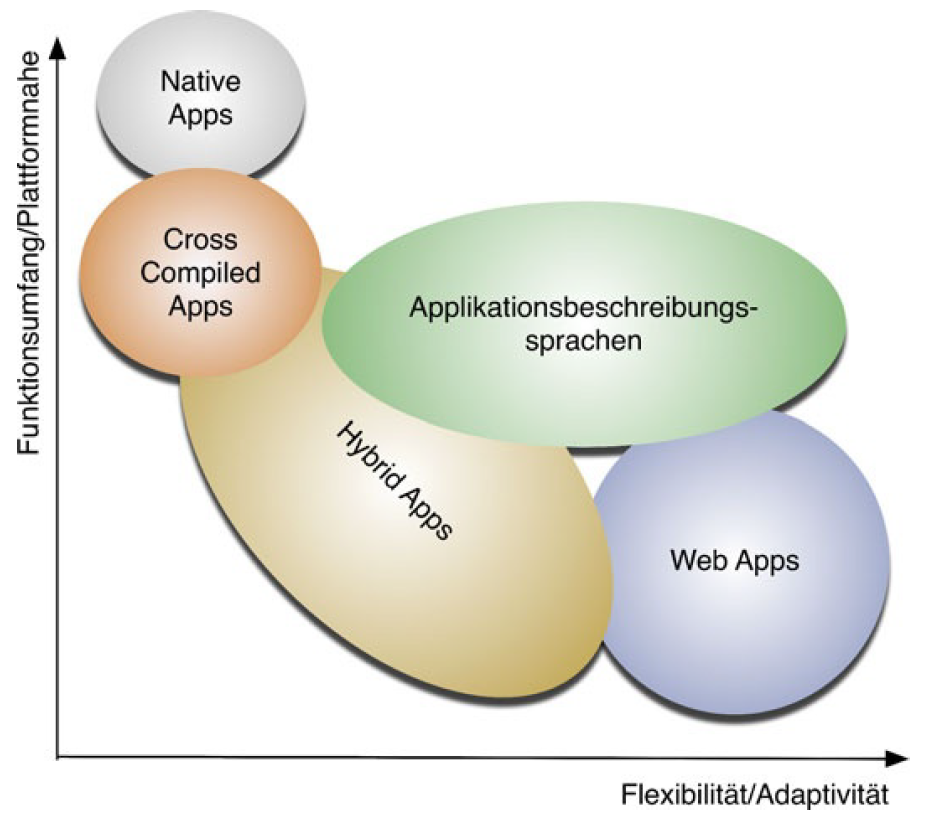
\includegraphics[width=0.8\linewidth]{images/apps_flexibilitaet_funktionsumfang.png}
	\caption{Übersicht über Arten von Applikationen nach Flexibilität und Funktionsumfang \cite[S.405]{Willnecker.2012}}
	\label{fig:appsFlexibilitaetFunktionsumfang}
\end{figure}


\subsubsection*{Aufbau}
Eine hybride App besteht in der Regel aus mehreren Teilen. Es gibt einen Kern, in dem sich der Quellcode für die eigentliche Applikation befindet und für Android und iOS jeweils einen Teil, in dem der native Code generiert wird. Der Kern der App wird häufig mit Web-Technologien erstellt. Dabei kann es sich z.\,B. um HTML, CSS und JavaScript handeln. Es können allerdings auch abweichende Sprachen (z.\,B. Dart oder C\#) zum Einsatz kommen.

Frameworks für hybride Apps liefern eine JavaScript-Bridge mit, welche den eigentlichen Quellcode in nativen Code umwandelt. Dieser wird dann zur Erstellung von Android- bzw. iOS-Apps genutzt. Wurde der native Code erstellt, kann man diesen über die jeweilige Entwicklungsumgebung öffnen und wie den Quellcode einer nativen App verwenden.

Da eine hybride App oft unter dem Slogan \glqq{}write once, run everywhere\grqq\:beworben wird, ist es notwendig, die Applikation unabhängig vom konkreten Betriebssystem auf gleiche Art und Weise anzuzeigen. Um dies zu erreichen, wird häufig in der App eine Webview angezeigt, welche den JavaScript-Code wiedergibt.

\begin{displayquote}
    \glqq Hybrid app looks and performs in native way but works like web app, so hybrid app possesses the great user experience of native app and cross-platform characteristic of web app at the same time.\grqq{}\\
    ~\cite{Que.2016}
\end{displayquote}


\subsection{Vor- und Nachteile}
Hybride Applikationen bringen einige Vor- und Nachteile mit sich, die in diesem Abschnitt genauer betrachtet werden. Abschließend wird ein Fazit getroffen und die wichtigsten Aussagen zusammengefasst.

\subsubsection*{Vorteile}
Der zentrale Vorteil hybrider Applikationen besteht in der Kompatibilität zu verschiedenen Betriebssystemen. Gemäß dem \glqq Write once, run anywhere\grqq-Paradigma ist die gemeinsame Codebasis mit den meistverwendeten, mobilen Betriebssystemen kompatibel \cite{Denko.2021}. Dabei handelt es sich Stand 2022 zu über 99\% um die Betriebssysteme Android und iOS \cite{Statista.06.11.2022}. Somit sind auch die Entwicklungskosten deutlich geringer als bei nativen Applikationen, da ein Entwicklungsteam für alle Betriebssysteme zeitgleich entwickeln kann \cite{Kleinschrod.2020}. Dies bietet sich besonders für Start-Up-Unternehmen an, die mit wenigen Mitarbeitern schnell eine funktionsfähige Applikation entwickeln wollen. Da hybride Applikationen somit auch in den beiden App Stores von Google und Apple angeboten werden können, kann eine höhere Anzahl potentieller Nutzer erreicht werden als bei nativen Applikationen, die auf eine konkrete Plattform beschränkt sind \cite{Tyshchenko.19.06.2020}. 

Da die Codebasis hybrider Applikationen mit Webtechnologien entwickelt wird, kommen im Entwicklungsprozess vergleichsweise einfach zu erlernende Programmiersprachen wie HTML, CSS und JavaScript zum Einsatz. Native Applikationen werden mit Java oder Kotlin für Android und Swift oder Objective-C für iOS entwickelt, wobei es sich jeweils um deutlich komplexere Programmiersprachen handelt \cite{Tyshchenko.19.06.2020}. Der Zugriff auf die Sensoren des Endgeräts (z.\,B. GPS, Kamera oder Beschleunigungssensor) ist bei hybriden Applikationen durch Verwendung einer Bridge zu den Schnittstellen des Betriebssystems möglich \cite{Que.2016}, wobei es sich um einen klaren Vorteil gegenüber Web-Applikationen handelt. Außerdem können hybride Applikationen genau wie native Applikationen Daten in lokalen Datenbanken abspeichern \cite{Denko.2021}. Sie sind somit auch offline verfügbar, was bei Web-Applikationen nicht der Fall ist.

\subsubsection*{Nachteile}
Hybride Applikationen haben grundsätzlich eine geringere Performance als native Applikationen und nutzen die Leistungsfähigkeit des Endgeräts nicht optimal aus \cite{Kleinschrod.2020}. Dies hat die Ursache, dass es durch die notwendige Kommunikation zwischen Applikation und nativen Komponenten zu Geschwindigkeitseinbußen kommt. Zudem ist es bei nativen Applikationen einfacher, die UX (User Experience) besser für jedes Betriebssystem zu optimieren, da direkt mit nativen Widgets gearbeitet werden kann \cite{Cowart.2012}. Bei hybriden Applikationen ist dies nicht der Fall, sodass die Entwicklung einer Benutzeroberfläche, die auf allen Plattformen gut aussieht, anspruchsvoll sein kann. Außerdem sind hybride Applikationen tendenziell anfälliger für Fehler und Ausfälle als native Applikationen \cite{Tyshchenko.19.06.2020}.

Ein weiterer Aspekt der Entwicklung hybrider Applikationen ist der Testprozess. Dieser ist grundsätzlich aufwändiger als bei nativen Applikationen, da die Applikation für alle Plattformen getestet werden muss. Dies erschwert auch die Testautomatisierung, da die Skripte einen größeren Funktionsumfang abdecken müssen \cite{Tyshchenko.19.06.2020}. Neben den Funktionstests (z.\,B. Ressourcenzugriff und Verhalten), Oberflächentests (z.\,B. korrekte Darstellung) und Leistungstests (z.\,B. Lasttest und Stresstest) gibt es zwei weitere Testarten, die besonders im Testprozess hybrider Applikationen relevant sind. Dabei handelt es sich um Kompatibilitätstests und Verbindungstests \cite{Tyshchenko.19.06.2020}. Kompatibilitätstests sind sinnvoll, um die korrekte Ausführung der hybriden Applikation auf mehreren Betriebssystemen sicherzustellen. Durch Verbindungstests wird das korrekte Verhalten der Applikationen online und offline sichergestellt.

\subsubsection*{Fazit}
Hybride Applikationen sind ein guter Kompromiss zwischen nativen Applikationen und Web-Applikationen. Sie kombinieren die wichtigsten Vorteile der beiden Applikationsarten und versuchen, daraus entstehende Nachteile bestmöglich zu reduzieren. Zusammengefasst kann man sagen, dass hybride Applikationen die schnelle, einfache und kostengünstige Entwicklung einer Applikation für mehrere Betriebssysteme ermöglichen und dafür eine leicht reduzierte Performance, eine etwas erschwerte Optimierung der Benutzeroberfläche und einen etwas aufwändigeren Testprozess in Kauf nehmen.


\subsection{Potential}
Trotz der einzugehenden Kompromisse gegenüber nativen Applikationen sind beliebte und vielverwendete hybride Applikationen bereits Bestandteil unseres Alltags und im Fokus von großen Unternehmen. Bekannte Beispiele für hybride Applikationen sind Twitter, Instagram, Evernote, Uber und Remote POS.

Diese Apps demonstrieren, dass die Leistungsfähigkeit von hybriden Applikationen durchaus den derzeitigen Anforderungen des Markts gewachsen sind und ein Interesse in der Verwendung und Weiterentwicklung von hybriden Frameworks besteht \cite{Dharmwan.27.04.2021}.

Die Möglichkeit, eine Applikation in den App Stores gängiger Anbieter zu veröffentlichen, ohne dass die Entwicklungskosten proportional zu der Anzahl der gewünschten Zielplattformen wachsen, ist ein Potential, das Firmen bei der Entwicklung ihrer Applikationen nutzen können und möchten.

\clearpage

\section{Vergleichskriterien}
% ca. 4 Seiten
In diesem Kapitel werden Vergleichskriterien ermittelt, anhand derer die Frameworks untersucht werden. Anschließend werden Anwendungsgebiete bestimmt und die Relevanz der Vergleichskriterien je Anwendungsgebiet gewichtet.

\subsection{Bestimmung}
%ca. 2 Seiten
Folgende Vergleichskriterien werden bei der Untersuchung der Frameworks berücksichtigt.

\textbf{Plattformspezifische Funktionen}\\
Die Zugriffsmöglichkeiten des Frameworks auf plattformspezifische Funktionen wird untersucht. Dies umfasst z.\,B. die Speicherverwaltung, die sich je nach Betriebssystem unterscheidet. Außerdem wird der Zugriff auf verschiedene Sensoren betrachtet. Dazu gehört u.\,A. die Standortermittlung durch GPS, der Umgebungslichtsensor oder das Magnetometer.

\textbf{Performance}\\
Die Performance des Frameworks wird u.\,A. mithilfe von Literatur bewertet. Dabei werden Geschwindigkeitseinbußen bei der Kommunikation zwischen Codebasis und dem nativen Wrapper, der plattformspezifische Funktionen realisiert, berücksichtigt. Zur detaillierten Bestimmung der Leistungswerte für die definierten Anwendungsgebiete sind Prototyping und Benchmarking notwendig. Ein weiterer Aspekt ist u.\,A. die Dateigröße des Builds für die jeweiligen Zielplattformen.

\textbf{Benutzeroberfläche}\\
Die Vorgehenweise bei der Erstellung der Benutzeroberfläche wird untersucht. Dabei wird betrachtet, in welchem Umfang grafische Elemente zur Verfügung stehen und durch welche strukturellen Elemente die responsive Anordnung der Elemente umgesetzt ist. Außerdem wird untersucht, welche Technologien (z.\,B. HTML \& CSS oder native Elemente) zur Entwicklung der Benutzeroberfläche eingesetzt werden.

\textbf{Erste Schritte}\\
Die Einrichtung des Frameworks wird betrachtet. Dabei wird untersucht, wie aufwändig und schwierig die Installation ist und ob weitere Abhängigkeiten zu dritten Programmen bestehen, die ebenfalls installiert werden müssen. Außerdem wird die Komplexität der Einarbeitung in das Framework bewertet, wobei z.\,B. Einstiegsschwierigkeiten hervorgehoben werden.  

\textbf{Entwicklungsunterstützung}\\
Die Unterstützung bei der Softwarentwicklung mit dem Framework wird bewertet. Dabei wird untersucht, welche IDEs verwendet werden können und ob dabei für die kommerzielle Verwendung kostenpflichtige Lizenzen benötigt werden. Außerdem wird betrachtet, ob es IDE-Erweiterungen für das Framework gibt und ob Templates für die Entwicklung existieren.

\textbf{Dokumentation}\\
Die Dokumentation des Frameworks wird bewertet. Dabei wird Wert auf den Umfang und die Nutzerfreundlichkeit der Dokumentation gelegt. Außerdem wird die Übersichtlichkeit und die Verfügbarkeit betrachtet.

\textbf{Ökosystem}\\
Das Ökosystem des Frameworks wird untersucht. Dabei wird die Vielzahl der zur Verfügung stehenden Klassenbibliotheken betrachtet, die den Funktionsumfang des Frameworks erweitern. Außerdem wird die Kompatibilität zu externen Diensten untersucht.

\textbf{Lebenszyklus \& öffentliches Interesse}\\
Der Lebenszyklus des Frameworks wird betrachtet. Es wird bewertet, wie populär und modern das Framework ist und an welchem Punkt des Lebenszyklus es sich befindet. So kann bestimmt werden, wie wahrscheinlich eine zeitnahe Einstellung der Weiterentwicklung des Frameworks ist und ob sich ein Umstieg auf die langfristige Softwareentwicklung mithilfe des Frameworks empfiehlt.

Außerdem werden folgende Aspekte betrachtet, die jedoch nicht Teil des anschließenden Vergleichs sind.

\begin{description}
    \item[Programmiersprachen] Programmiersprachen, in denen die Softwareentwicklung erfolgt
    \item[Zielplattformen] Zielplattformen, für die Software entwickelt werden kann
    \item[Wartbarkeit] Architektur-Patterns, die mithilfe des Frameworks umgesetzt werden können
    \item[Datenhaltung] DBMS, die vom Framework unterstützt werden
    \item[Lizenz \& Kosten] Lizenz, unter der das Framework steht und eventuell anfallende Kosten
\end{description}


\subsection{Anwendungsgebiete}\label{subsec:areas}
Um die Frameworks bestmöglich zu testen, müssen Anwendungsgebiete definiert werden, für die in den jeweiligen Frameworks beispielhaft hybride Applikationen erstellt werden. Diese Anwendungsgebiete werden im Folgenden näher beschrieben.

\subsubsection*{Formularlastige Anwendung}
Eine formularlastige Anwendung ist eine Anwendung, in welche Benutzer*innen Informationen über Formulare eingeben können. Diese Daten sollen beispielhaft in einer lokalen Datenbank abgespeichert und wieder daraus geladen werden. Außerdem wird bei der Entwicklung der Funktionsumfang und der Aufwand zur Erstellung der Formulare betrachtet. Auch die Usability soll ermittelt werden, indem notiert wird, was beim Ausfüllen der jeweiligen Formulare auffällt und was positiv bzw. negativ hervorzuheben ist.

\subsubsection*{Sensorlastige Anwendung}
Damit ein Smartphone mit der Umwelt kommunizieren kann, haben aktuelle Geräte eine große Anzahl an Sensoren eingebaut. Ein aktuelles Smartphone der Mittelklasse hat üblicherweise mindestens folgende Sensoren eingebaut:
\begin{description}
	\item[Gyroskop] Misst die Rotation des Geräts.
	\item[Beschleunigungssensor] Misst, ob das Gerät in Bewegung ist.
	\item[Lichtsensor] Misst die Helligkeit der Umgebung.
	\item[GPS-Sensor] Bestimmt die Position des Geräts.
	\item[Kamera] Aufnahme von Bildern und Videos.
	\item[Fingerabdrucksensor] Registriert den Fingerabdruck der Benutzer*in.
\end{description}
Um zu ermitteln, welche Sensoren das jeweilige Framework nutzen kann, soll eine Applikation entwickelt werden, welche diese Sensoren im Einsatz zeigt. Hierbei soll auch berücksichtigt werden, wie einfach es ist, die Messungen der Sensoren in der Applikation zu berücksichtigen.

\subsubsection*{Rechenintensive Anwendung}
Um die Leistung der Frameworks zu messen, sollen rechenintensive Funktionen implementiert werden. Hierbei soll ermittelt werden, wie lange das Framework für die Berechnungen benötigt und wie stark die CPU ausgelastet wird. Außerdem soll ermittelt werden, wie das Framework mit Extremsituationen wie einem hohen Leistungsbedarf zurechtkommt und ob es vielleicht sogar ab einem gewissen Grad abstürzt.

\subsection{Gewichtung} \label{sec:gewichtung}
%ca. 1 Seite
Die Anforderungen an eine Applikation variieren von Anwendungsgebiet zu Anwendungsgebiet. Um dies im Vergleich zu berücksichtigen, erfolgt eine individuelle Gewichtung der Vergleichskriterien je Anwendungsgebiet. Im Rahmen eines paarweisen Vergleichs werden die Vergleichskriterien systematisch gegenübergestellt und entschieden, welches der betrachteten Kriterien wichtiger ist. Die Summe der gewonnenen Vergleiche wird durch die Anzahl der Vergleichskriterien geteilt, um eine prozentuale Gewichtung des betrachteten Vergleichskriteriums zu erhalten.

Im Folgenden werden die paarweise Vergleiche und die daraus resultierende Gewichtung der Vergleichskriterien für die Anwendungsgebiete dargestellt und Auffälligkeiten aufgezeigt.

\subsubsection{Formularlastige Anwendung}

\begin{figure}[h]
	\centering
	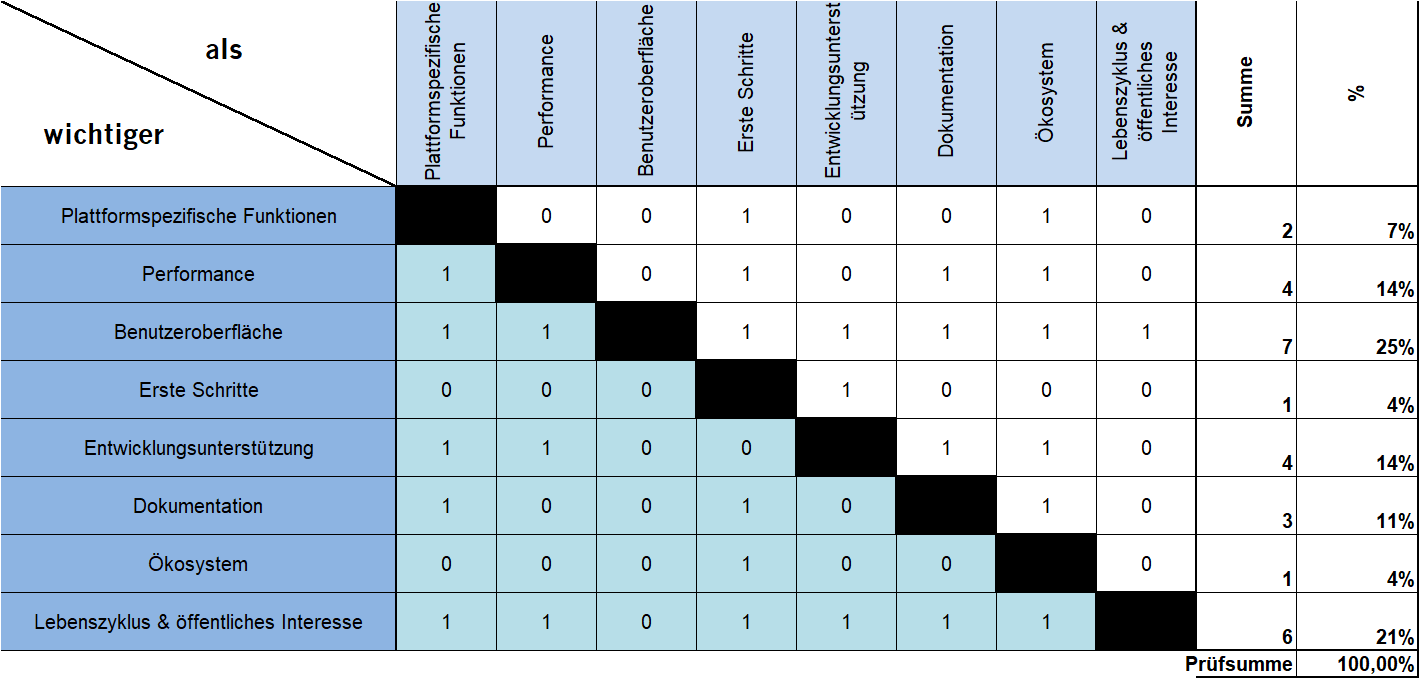
\includegraphics[width=0.85\linewidth]{images/GewichtungFormularlastig.png}
	\caption{Gewichtung der Kriterien in formularlastigen Anwendungen}
	\label{fig:weightFormula}
\end{figure}

In Abbildung \ref{fig:weightFormula} ist der paarweise Vergleich und die daraus resultierende Gewichtung der Vergleichskriterien für das Anwendungsgebiet der formularlastigen Anwendungen dargestellt. Die Benutzeroberfläche wurde wichtiger als alle sieben verbleibenden Vergleichskriterien eingestuft und erhält dadurch eine relative Gewichtung von 25\%. Der Lebenszyklus und das öffentliche Interesse erhält eine relative Gewichtung von 21\%. Performance und Entwicklungsunterstützung erhalten jeweils eine relative Gewichtung von 14\%. Erste Schritte und Ökosystem erhalten jeweils eine relative Gewichtung von 4\%.

\subsubsection{Sensorlastige Anwendung}

\begin{figure}[h]
	\centering
	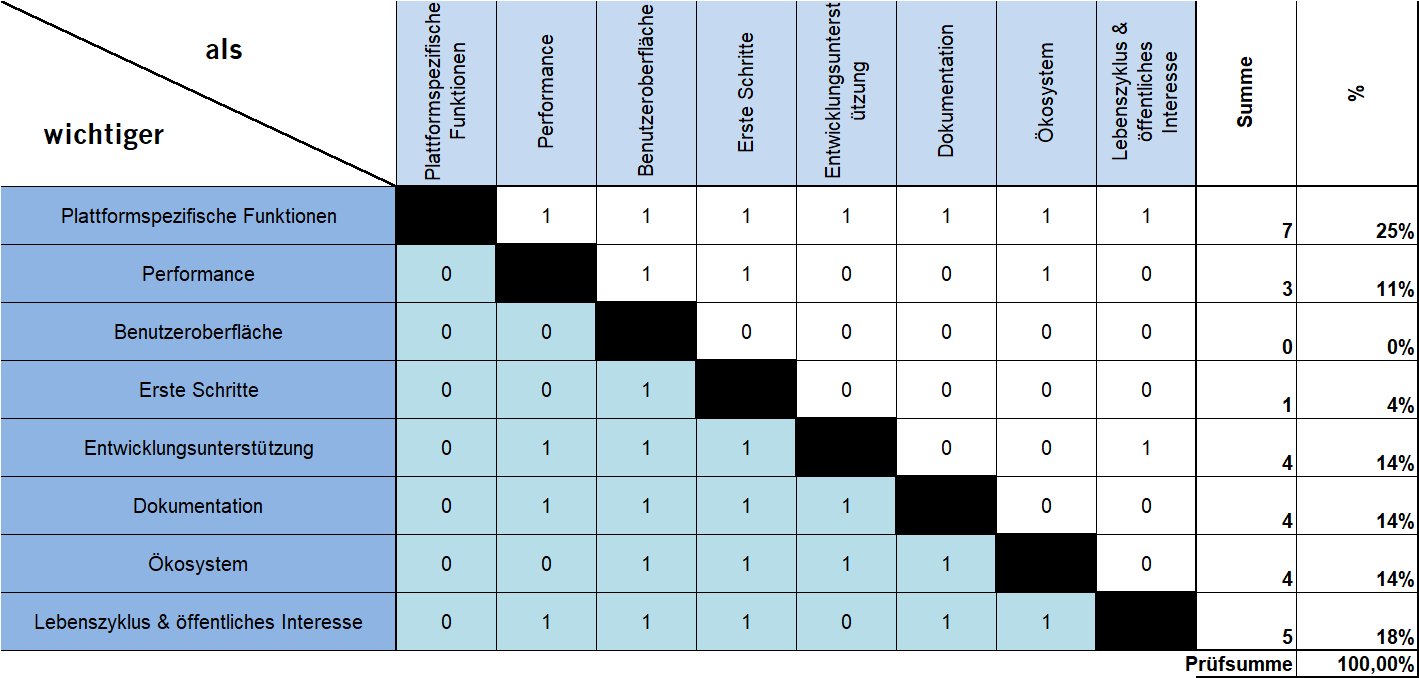
\includegraphics[width=0.85\linewidth]{images/GewichtungSensorlastig.png}
	\caption{Gewichtung der Kriterien in sensorlastigen Anwendungen}
	\label{fig:weightSensor}
\end{figure}

In Abbildung \ref{fig:weightSensor} ist der paarweise Vergleich und die daraus resultierende Gewichtung der Vergleichskriterien für das Anwendungsgebiet der sensorlastigen Anwendungen dargestellt. Die plattformspezifische Funktionen wurde wichtiger als alle sieben verbleibenden Vergleichskriterien eingestuft und erhalten dadurch eine relative Gewichtung von 25\%. Der Lebenszyklus und das öffentliche Interesse erhält eine relative Gewichtung von 18\%. Entwicklungsunterstützung, Dokumentation und Ökosystem erhalten jeweils eine relative Gewichtung von 14\%. Alle Vergleichskriterien wurden wichtiger als die Benutzeroberfläche eingestuft, diese erhält dadurch eine relative Gewichtung von 0\%.

\subsubsection{Rechenintensive Anwendung}

\begin{figure}[h]
	\centering
	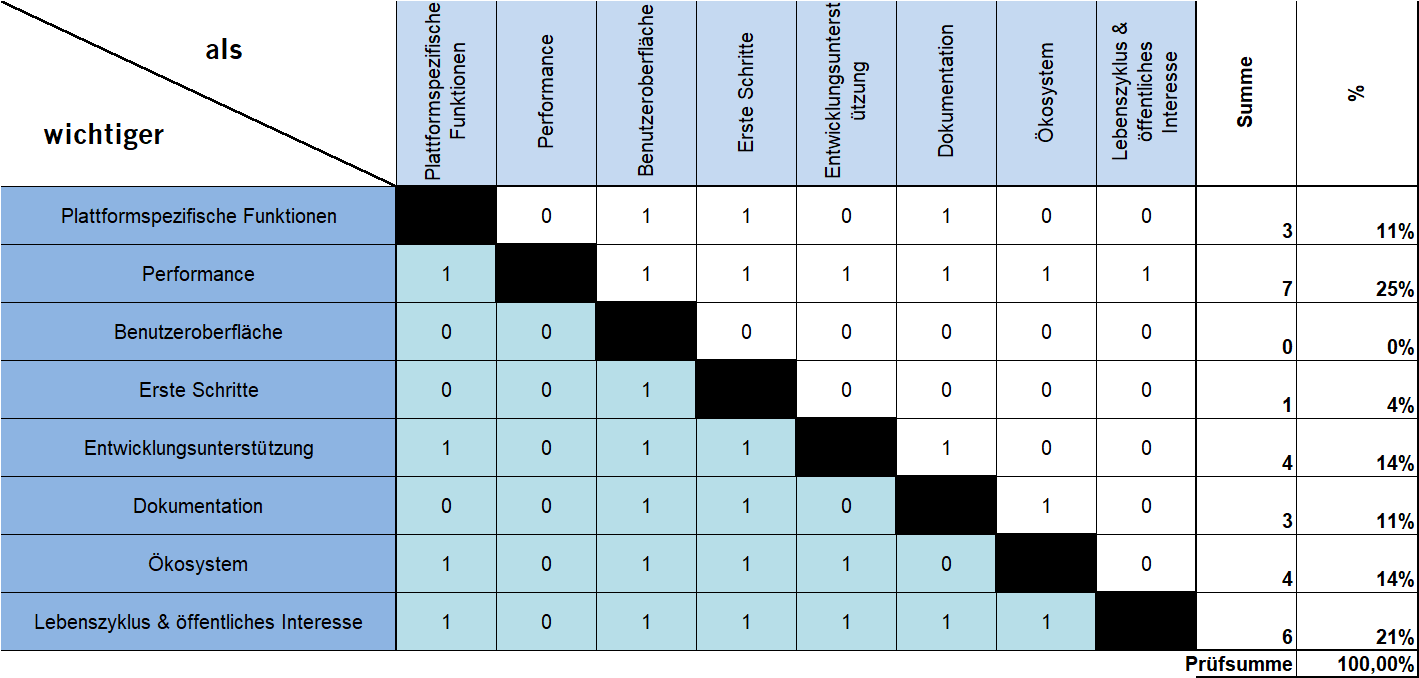
\includegraphics[width=0.85\linewidth]{images/GewichtungRechenintensiv.png}
	\caption{Gewichtung der Kriterien in rechenintensiven Anwendungen}
	\label{fig:weightCalc}
\end{figure}

In Abbildung \ref{fig:weightCalc} ist der paarweise Vergleich und die daraus resultierende Gewichtung der Vergleichskriterien für das Anwendungsgebiet der rechenintensiven Anwendungen dargestellt. Die Performance wurde wichtiger als alle sieben verbleibenden Vergleichskriterien eingestuft und erhält dadurch eine relative Gewichtung von 25\%. Der Lebenszyklus und das öffentliche Interesse erhält eine relative Gewichtung von 21\%. Entwicklungsunterstützung, sowie Ökosystem, erhalten jeweils eine relative Gewichtung von 14\%. Alle Vergleichskriterien wurden wichtiger als die Benutzeroberfläche eingestuft, diese erhält dadurch eine relative Gewichtung von 0\%.

\subsubsection{Auffälligkeiten}
Bei der Betrachtung der Ergebnisse fällt auf, dass Lebenszyklus und öffentliches Interesse bei jedem Anwendungsgebiet als zweitwichtigstes Kriterium gewichtet ist. Außerdem ist erkannbar, dass die Benutzeroberfläche hauptsächlich bei formularlastigen Anwendungen relevant und bei rechenintensiven und sensorlastigen Anwendungen zu vernachlässigen ist. In jedem Anwendungsgebiet dominiert ein Vergleichskriterium mit 25\%, welches repräsentativ für die Anforderungen des Anwendungsgebiets ist.

\clearpage

\section{Hybride Frameworks} \label{sec:frameworks}
% ca. 10 Seiten
In diesem Kapitel werden Frameworks zur Entwicklung hybrider Applikationen untersucht. Dabei werden die Kriterien aus dem vorherigen Kapitel berücksichtigt.

\subsection{Flutter}
%Jannik (<= 2 Seiten)
Flutter ist ein modernes, hybrides Framework, das von Google entwickelt und 2018 veröffentlicht wurde. Als Open-Source-Framework steht unter der BSD-Lizenz und ist somit in kommerziellen Projekten nutzbar. Die Entwicklung erfolgt in der objektorientierten Programmiersprache Dart, die als Nachfolger von JavaScript entwickelt wurde und viele der charakteristischen JavaScript-Funktionalitäten implementiert, sich dabei allerdings eher an der Syntax von Java orientiert \cite{Wu.2018}. Außerdem können Bibliotheken in den Programmiersprachen C und C++ eingebunden werden. Mit Flutter können Applikationen für Android, iOS, Windows, Linux, macOS und Browser wie Firefox, Chrome oder Edge entwickelt werden.

Obwohl Flutter ein vergleichsweise neues und modernes Framework ist, zeichnet es sich durch eine detaillierte und umfangreiche Dokumentation aus. Diese deckt den gesamten Entwicklungsprozess ab und leitet den Entwickler von der Installation bis zum Deployment der Flutter-Applikationen. Außerdem sind Beispielprojekte und Videoanleitungen auf dem Youtube-Kanal von Flutter zu finden. Die Dokumentation ist online \footnote{https://docs.flutter.dev/} einsehbar und steht bei Bedarf ebenfalls als Download \footnote{https://api.flutter.dev/offline/flutter.docset.tar.gz} zur Verfügung. Zum aktuellen Zeitpunkt ist sie ausschließlich auf Englisch verfasst. 

Flutter ist für die Plattformen Windows, macOS, Linux und ChromeOS verfügbar. Zur Installation muss das FlutterSDK inklusive der enthaltenen Dart Virtual Machine heruntergeladen, extrahiert und im gewünschten Verzeichnis abgelegt werden. Flutter benötigt mehrere Abhängigkeiten zu anderen Programmen. Diese können mithilfe des Befehls \emph{flutter doctor} in der Konsole abgefragt werden. Konkret werden Android SDK, Android Studio, Visual Studio, Visual Studio Code, IntelliJ IDEA und Chrome benötigt. Außerdem werden sogenannte Host Devices benötigt, auf denen das Debugging der Applikationen stattfinden kann. Für Android können diese im Android Emulator von Android Studio konfiguriert werden. Dazu ist es jedoch notwendig, die VM Hardware Acceleration zu aktivieren, was einen gewissen Aufwand mit sich bringt. Genaue Anweisungen sind in der Flutter Dokumentation zu finden.

Die Entwicklung von Flutter-Applikationen kann in verschiedenen IDEs (Integrierte   Entwicklungsumgebung) erfolgen. Visual Studio Code ist die populärste IDE, da sie auch in kommerziellen Projekten kostenlos nutzbar ist und mit der \emph{Flutter Extension} weitere Funktionalitäten zur Bearbeitung, Refactoring und Ausführung der Applikationen hinzugefügt werden können. Weitere IDEs sind z.\,B. Android Studio oder IntelliJ IDEA. Besonders hervorgehoben werden muss die Hot-Reload-Funktion von Flutter, die ein schnelles Nachladen bei Änderungen während der Ausführung der Applikation ermöglicht und auch bei größeren Änderungen noch zuverlässig und schnell funktioniert. Dies geschieht durch Injection der modifizierten Code-Dateien in die laufende Dart Virtual Machine \cite{Zammetti.2019}. Außerdem stehen für Flutter hunderte Templates auf diversen Websites \footnote{z.\,B. https://flutterawesome.com/tag/templates/} zur Verfügung, die die Entwicklung deutlich beschleunigen können und viele Anwendungsgebiete bereits abdecken.  

Flutter ermöglicht einen einfachen Zugriff auf spezifische Funktionen der jeweiligen Zielplattform. Mithilfe von Paketen  (z.\,B. \emph{sensors\_plus} oder \emph{flutter\_sensors}) kann auf die Sensoren des Endgeräts wie z.B. Beschleunigungssensor, Gyroskop, Magnetometer, Näherungssensor und viele mehr zugegriffen werden. Außerdem ist es möglich, den Zugriff auf plattformspezifische Schnittstellen selbst in Dart zu implementieren, um z.\,B. den Akkustand abzufragen. Die Speicherverwaltung der Applikationen liegt nicht in der Hand des Entwicklers, sondern wird von der Dart Virtual Machine übernommen, die u.\,A. einen Garbage Collector für die Freigabe von nicht mehr benötigtem Speicherplatz umfasst.

Die Benutzeroberfläche wird in Flutter modular, d.\,h. in Form von Komponenten, entwickelt. Dabei verwendet Flutter nicht wie die meisten Frameworks OEM (Original Equipment Manufacturer)-Widgets, die vom Betriebssystem des Endgeräts zur Verfügung gestellt werden, sondern generiert eigene Widgets. Dies ermöglicht ein einzigartiges Design der Widgets und erhöht die Erweiterbarkeit und Flexibilität \cite{xster.16.11.2017}. Für die Umsetzung der Benutzeroberfläche wird die Komponente \emph{MaterialApp} als Top-Level-Widget verwendet, da sie z.\,B. Kopfzeile und Navigator bereits enthält. Die Oberfläche ist üblicherweise als Grid-Struktur organisiert, sodass die Anordnung der Widgets in Reihen (Row) und Spalten (Column) möglich ist. Für das Styling ist kein CSS (Cascading Style Sheets) notwendig, da die Gestaltung mithilfe von Decoration- und Style-Elementen direkt in Dart erfolgen kann. Zu diesem Zweck stehen auch weitere Elemente wie Center(), Positioned() oder Transform() zur Verfügung, um die Widgets innerhalb der Grid-Zelle auszurichten.

Da Flutter nicht die OEM-Widgets des Betriebssystems verwendet, kann in der Regel eine höhere Performance als bei anderen Frameworks erreicht werden. Dies hat den Hintergrund, dass Geschwindigkeitseinbußen, die durch die Kommunikation zwischen Applikation und nativen Komponenten entstehen würden, vermieden werden können \cite{HeliosBlog.2020}. Stattdessen nutzt Flutter seine eigene Hochleistungsengine Skia zum Rendern der benötigten Widgets \cite{Wu.2018}. Man spricht daher davon, dass das Rendering von der Systemebene in die Applikationsebene verlagert wird. Dies führt allerdings dazu, dass die Build-Dateien größer als bei anderen Frameworks sind, da die eigenen Widgets und Renderer ebenfalls in der releasten Applikation enthalten sein müssen \cite{Wu.2018}. Grundsätzlich ist Dart als eine Programmiersprache mit hoher Performance zu betrachten, da sowohl JIT (Just-in-Time)-Kompilierung für die Entwicklung als auch AOT (Ahead-of-Time)-Kompilierung für den Release der Applikation eingesetzt werden \cite{DartDocumentation.02.11.2022}. AOT-kompilierter Code ermöglicht einen schnellen Start des Programms und zuverlässig geringe Ausführungszeiten während des gesamten Programmablaufs \cite{Obinna.07.04.2020}.

Im Flutter-Ökosystem steht eine große Anzahl an Paketen zur Verfügung. Dabei ist nahezu jeder Bereich von Datenbanken über WebSockets und Audio bis hin zu Animationen abgedeckt. Zur Organisation wird das offizielle Paket-Repository pub.dev verwendet. Von dort können die Pakete über den Pub Package Manager einfach in eigene Projekte integriert werden, indem die Dependency mit der benötigten Version in einer Projektdatei hinterlegt wird und dann beim nächsten Build aufgelöst wird. Anschließend kann das Paket mithilfe des import-Befehls verwendet werden.

Für die Datenhaltung steht eine recht begrenzte, aber wachsende Auswahl an Datenbanksystemen zur Verfügung. Die Pakete sqflite und moor erlauben den Zugriff auf das relationale Datenbanksystem SQLite, indem sie als Wrapper speziell für Flutter fungieren und SQL-Queries sowohl in SQL als auch direkt in Dart ermöglichen. Der Zugriff auf NoSQL Datenbanksysteme ist ebenfalls möglich. Zu diesem Zweck können die Pakete hive und firebase verwendet werden, die Unterstützung für die gleichnamige Key-Value-Datenbank und JSON-Datenbank bieten \cite{Greenrobot.2021}.

Flutter steht seit seinem Release in Konkurrenz mit dem Framework \hyperref[sec:ReactNative]{React Native}. Es ist nicht eindeutig absehbar, welches Framework sich langfristig durchsetzen wird. Allerdings gewinnt Flutter in den letzten Jahren immer weiter Marktanteile und ist seit 2021 das meistverwendete, hybride Framework am Markt \cite{Statista.21.10.2022}. Der Umstieg von Unternehmen auf die Softwareentwicklung mit Flutter scheint daher langfristig sinnvoll, da es sich voraussichtlich weiterhin als eines der meistverwendeten Frameworks etablieren wird.


\subsection{React Native} \label{sec:ReactNative}
React Native wurde im Jahr 2015 von Meta entwickelt und bis zum Jahr 2020 so weiterentwickelt, dass es ausgereift und für den Einsatz im Produktivumfeld geeignet ist. React Native begann als internes Hackathon-Projekt, dabei war das eigentliche Ziel des Projekts, den Entwicklungsprozess von Android und iOS zu vereinheitlichen \cite{Niemeier.04.11.2022}. Das Framework ist Open-Source und steht unter der MIT-Lizenz. Aufgrund dieser Lizenz kann das Framework auch kommerziell verwendet werden. Es unterstützt die wichtigsten mobilen Plattformen Android und iOS genauso wie Windows, macOS und AndroidTV. Nicht zuletzt unterstützt es natürlich auch das Entwickeln von Webanwendungen. Viele namhafte Applikationen setzen bereits React Native ein, darunter sind Anwendungen wie Instagram, Skype oder auch Uber Eats \cite{Chandratre.28.01.2020}.

Die Entwicklung einer App in React Native erfolgt auf Basis von Webtechnologien wie HTML, CSS und JavaScript \cite{Zammetti.2019}. Das Framework setzt unter Anderem auch die verwandte JavaScript-Bibliothek ReactJS ein, welche auch von Meta entwickelt wurde. Der Unterschied zwischen React und React Native ist, dass React auf die Entwicklung von Web-Applikationen spezialisiert ist, während React Native für die Entwicklung von nativen Apps optimiert ist \cite{Lestal.12.08.2020}. Entwickler, die bereits in React Anwendungen entwickelt haben, können diesen Code auch weiterhin nutzen \cite{Krypczyk.2021}.

React Native kann schnell und einfach eingerichtet werden. Für die Entwicklungsumgebungen von Jetbrains gibt es Plugins, welche ganz bequem über das Plugin-Portal installiert werden können. Genauso gibt es auch für Visual Studio Code aus dem Hause Microsoft Unterstützung durch Plugins. Um React Native zu installieren, muss zuerst NodeJS und NPM installiert werden. NodeJS ist ein Framework, welches die Entwicklung von JavaScript-Anwendungen erleichtert. Über NPM können andere Bibliotheken per Kommandozeilenbefehl installiert werden. Für React Native gibt es auch ein sogenanntes Command Line Interface. Über dieses Interface kann man das System auf einfache Weise aktualisieren oder Erweiterungen installieren. Ist NPM installiert, so kann durch Aufrufen bestimmter Befehle in der Kommandozeile das Framework installiert und eine Anwendung eingerichtet werden. Da der Code von React Native in nativen Code umgewandelt wird, müssen für Android und iOS ebenso auch die nativen Entwicklungsumgebungen installiert werden. Dies wären Android Studio für Android und AppCode für iOS. Über diese nativen Entwicklungsumgebungen kann man auch Emulatoren der jeweiligen Betriebssysteme starten und so die App auf den Geräten testen \footnote{https://www.tutorialspoint.com/react\_native/react\_native\_environment\_setup.htm}.

Projekte in React Native bestehen aus Code, welcher in JavaScript erstellt wird. Dieser ist in Views unterteilt, welche die Oberfläche widerspiegeln und Services, welche die Fachlogik enthalten. Oberflächen werden in React entwickelt, die Geschäftslogik wird in JavaScript verfasst. Nach dem Build der Anwendung werden Views in native Views umgewandelt. Services nutzen über eine Bridge die Schnittstellen der nativen Plattformen \cite{Krypczyk.2021}. React Native unterstützt den Hot-Reloading Mechanismus, sodass Änderungen im Programmcode zur Laufzeit durchgeführt werden können, ohne dass die Anwendung neu gestartet werden muss. Jede React Native Anwendung besteht hauptsächlich aus zwei unterschiedlichen Arten von Threads. Dabei kümmert sich einer der Threads als Haupt-Thread um die Anzeige der Elemente in der Benutzeroberfläche, während der andere Thread für die Ausführung des JavaScript-Codes verantwortlich ist. Er definiert außerdem die Funktionalitäten der Elemente auf der Benutzeroberfläche \cite{Niemeier.04.11.2022}.

Da React Native Open-Source ist, gibt es viele Bibliotheken und Erweiterungen von anderen Entwicklern. Daher gibt es auch Bibliotheken, welche React Native um die Nutzung von Sensoren erweitern \cite{Schmidt.14.05.2018}. So werden z.\,B. Geschwindigkeitssensor, Gyroskop, Magnetometer und Barometer unterstützt. Über eine gut dokumentierte, native Schnittstelle werden auch native Elemente für die Oberfläche unterstützt. Dabei kann es sich z.\,B. um diverse Views in Android handeln.

In einer Datei können verschiedene Views hinterlegt werden, welche die Oberflächen der Applikation definieren. Views können sich auch je nach Plattform unterscheiden, sodass eine App auf Android später anders aussehen kann als auf iOS. Die einzelnen Views können modular aufgebaut werden und aus verschiedenen Dateien bestehen.

React Native unterstützt sehr viele Technologien und Schnittstellen, welche häufig bei der App-Entwicklung benötigt werden. So kann grundsätzlich auf native Oberflächenelemente zugegriffen werden. Der grundlegende Funktionsumfang kann beliebig durch eine der zahlreichen Erweiterungen ergänzt werden. Zum Beispiel kann durch Erweiterungen die Unterstützung für folgende Datenbank-Systemen ermöglicht werden: Firebase, SQLite, Realm, PouchDB, AsyncStorage und Weitere.

Zusammenfassend kann festgehalten werden, dass React Native voraussichtlich noch länger unterstützt wird, da hinter dem Framework eine namhafte Firma wie Meta steht. Das Projekt wird auf Open-Source-Basis entwickelt und kann so potenziell von jedem Entwickler weiterentwickelt werden. React Native hat einen großen Funktionsumfang und kann durch zusätzliche Erweiterungen dynamisch ausgebaut werden. Applikationen werden einmal gebaut und können für eine Vielzahl von Plattformen entwickelt werden. Um native Apps zu testen, müssen allerdings auch Entwicklungsumgebungen für die jeweiligen Plattformen installiert sein.


\subsection{.NET MAUI}\label{sec:MAUI}
%Ruben (<= 2 Seiten)
.NET MAUI (Multi-Platform App UI) ist ein Framework von Microsoft, mit dem seit 2022 plattformunabhängige Applikationen entwickelt werden können. MAUI ist der offizielle Nachfolger von Xamarin und verwendet bei linuxbasierten Zielplattformen ebenfalls die Laufzeitumgebung Mono \cite{Davidbritch.04.12.2022c}. 

Mit MAUI können Applikationen für Android, iOS, Windows, macOS und Tizen entwickelt werden. Die gemeinsame Codebasis wird in der objektorientierten Programmiersprache C\# geschrieben. Die Benutzeroberfläche kann wahlweise über die XML-basierte Beschreibungssprache XAML (Extensible Application Markup Language) oder unter Verwendung des Single-Page Web-Frameworks .NET Blazor erstellt werden. Bei letzterem spricht man von MAUI Blazor oder auch Blazor Hybrid, welches die Zielplattform um die gängigen Browser wie Chrome, Firefox und Edge erweitert.

Die Benutzeroberfläche wird in MAUI Blazor modular, d.\,h. in Form von wiederverwenbaren, dynamischen Komponenten entwickelt. Bei einer Razor-Komponente handelt es sich um einen eigenständigen Teil der Benutzeroberfläche und die dazugehörige Verarbeitungslogik. Die Komponenten werden in einer Kombination aus C\#, HTML-Markup und optionalem JavaScript implementiert. C\# ersetzt hierbei das bei Web-Frameworks üblicherweise benötigte JavaScript, sodass keine Kenntnisse über JavaScript benötigt werden. Die Darstellungsvorgaben können über CSS beliebig definiert werden. Sowohl einzelne Seiten als auch die komplette Blazor Applikation lassen sich über ein BlazorWebView-Steuerelement in der MAUI Applikation hosten. Die Web-UI wird anschließend in dem eingebetteten Steuerelement gerendert und die Komponenen werden im systemeigenen Prozess ausgeführt \cite{Davidbritch.04.12.2022}.

MAUI unterliegt der MIT-Lizenz und Blazor unterliegt der Apache-2.0-Lizenz, somit handelt es sich um Open-Source Software.

Obwohl MAUI und Blazor vergleichsweise neue Frameworks sind, zeichnen sie sich durch eine detaillierte und umfangreiche Dokumentation aus. Diese deckt den gesamten Entwicklungsprozess ab und leitet Entwickler*innen von der Installation bis zum Deployment der hybriden Applikation. Außerdem sind Beispielprojekte und Videoanleitungen auf der Lernplatform \footnote{https://dotnet.microsoft.com/en-us/learn/maui} und dem Youtube-Kanal von Microsoft und dotnet zu finden. Die Dokumentation ist online \footnote{https://learn.microsoft.com/de-de/aspnet/core/blazor/hybrid/?view=aspnetcore-6.0} einsehbar und verweist auf weitere nützliche Ressourcen. Zum aktuellen Zeitpunkt ist sie auf Englisch und auf Deutsch verfasst. 

Die Entwicklung von MAUI Applikationen kann in verschiedenen IDEs erfolgen. Visual Studio 2022, Visual Studio 2022 für Mac, Visual Studio Code und Rider sind namhafte Vertreter. Mit wenigen Schritten kann die bestehende Visual Studio Installation um den .NET MAUI Entwicklungsworkload erweitert werden. Hierzu werden weder Konsolenbefehle noch die manuelle Installation von weiteren Programmen benötigt. Der in Visual Studio enthaltene Android Emulator ermöglicht das Verwalten und Debuggen der simulierten Geräte, ohne die Entwicklungsumgebung zu verlassen. Um die Zielplattformen macOS und iOS zu Debuggen, wird ein Mac benötigt, welcher remote in die Entwicklungsumgebung eingebunden werden kann. Visual Studio ermöglicht ebenfalls Hot Reloading. Durch die Verwendung von Templates kann der Entwicklungsprozess beschleunigt werden \cite{Davidbritch.04.12.2022b}. 

Für MAUI und Blazor als Teile des .NET-Ökosystems gibt es viele Bibliotheken und Erweiterungen von anderen Entwicklern. Diese können unkompliziert über die Paketverwaltung NuGet eingebunden werden. Durch Blazors Interoperabilität zu JavaScript ist es ebenfalls möglich, JavaScript-Bibliotheken einzubinden. Für Sensoren, die weder über die MAUI-API noch über Bibliotheken angesprochen werden können, besteht die Möglichkeit, plattformspezifischen Code aus der gemeinsamen Codebasis aufzurufen. Für diese plattformbedingte Kompilierung werden entsprechende Kentnisse über die Schnittstellen der Zielplattform benötigt \cite{Davidbritch.06.11.2022}. 

MAUI vereint plattformspezifische Frameworks in einer einzigen API. Die geteilte Codebasis interagiert überwiegend mit der zielplattformunabhängigen MAUI-API, welche anschließend die spezifischen APIs der Zielplattformen konsumiert. Ein direkter Aufruf von Schnittstellen der Zielplattformen ist ebenfalls möglich. Abhängig von der Zielplattform wird wahlweise Ahead-of-Time (AOT) und Just-in-Time (JIT) Kompilierung ermöglicht \cite{Davidbritch.04.12.2022c}. In Abbildung \ref{fig:mauiOverview} ist die Architektur einer MAUI Applikation dargestellt.

\begin{figure}[h]
	\centering
	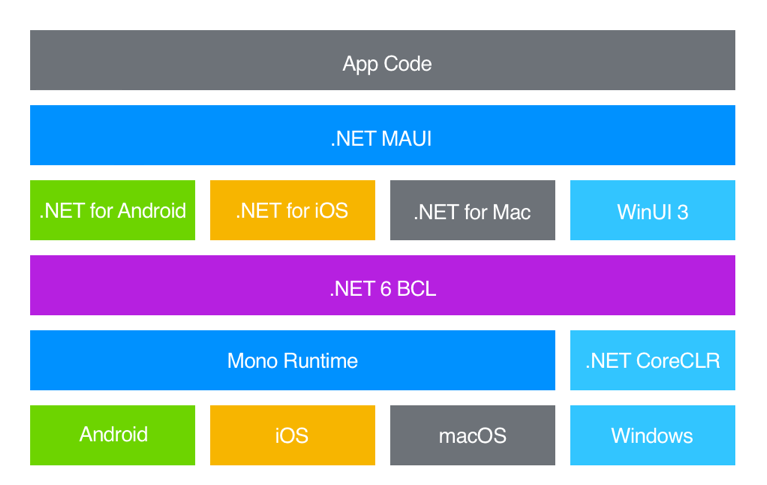
\includegraphics[width=0.8\linewidth]{images/maui_overview.png}
	\caption{Übersicht über die Architektur einer MAUI Applikation nach \cite{Davidbritch.04.12.2022c}}
	\label{fig:mauiOverview}
\end{figure}

Zusammenfassend kann festgehalten werden, dass die Entwicklung des Frameworks noch weiter voran geht und als Nachfolger von Xamarin auch entsprechend lange unterstützt wird. MAUI hat einen großen Funktionsumfang und kann durch zusätzliche Erweiterungen dynamisch ausgebaut werden. Durch die Möglichkeit, XAML oder Blazor einzusetzen, richtet sich MAUI sowohl an Webentwickler*innen, als auch an Entwickler*innen mit Erfahrung in Desktop-Applikationen.

\clearpage

\section{Vergleich der Frameworks}\label{sec:compare}
Im folgenden Kapitel wird der Vergleich der Frameworks durchgeführt. Dabei wird zunächst jedes Framework anhand der ermittelten Vergleichskriterien bewertet. Zur Bestimmung der Performance findet ein Benchmarking statt, bei dem Berechnungszeiten und CPU-Auslastung für rechenintensive Funktionen dokumentiert werden. Anschließend kann mit den Bewertungen und den zuvor bestimmten Gewichtungen für die Kriterien in jedem definierten Anwendungsgebiet eine Punktzahl errechnet werden, anhand derer die Frameworks sortiert werden können.

\subsection{Prototypen} \label{sec:prototypen}
% (2 Seiten)
Im Rahmen des Vergleichs werden für jedes Framework drei unterschiedliche Prototypen umgesetzt (vgl. Abschnitt \ref{subsec:areas}). Zur Demonstration einer formularlastigen App wird eine To-Do-Listen Applikation umgesetzt. Diese nimmt Aufgaben per Formular auf und speichert sie in einer lokalen Datenbank ab. Außerdem können Aufgaben gelöscht oder als \glqq{}erledigt\grqq{} markiert werden.\\
Die zweite Applikation ist eine sensorlastige App. Hierbei werden die gängigsten Sensoren über das Framework angesprochen und die Daten ausgelesen. Wichtig sind hierbei Sensoren wie z.\,B. der Beschleunigungssensor, das Gyroskop oder das Magnetometer.\\
Um die Performance zu vergleichen, wurden bei der rechenintensiven App eine rekursive und eine iterative Funktion implementiert. Bei der rekursiven Funktion handelt es sich um die Ackermann-Funktion. Diese ist dafür bekannt, sehr stark anzusteigen und die Rechenkapazität schnell zu erschöpfen. Die Ackermann-Funktion ist im Folgenden definiert \cite{Tutego.10.02.2015}.

\begin{lstlisting}[label={lst:Ackermann-Funktion}]
a(0,m) = m + 1
a(n,0) = a(n - 1, 1)
a(n,m) = a(n - 1, a(n, m - 1))
\end{lstlisting}

Als iterative Funktion dient eine Implementierung der Potenzierung, bei der die Berechnung der potenzierten Zahl iterativ erfolgt. Hierbei werden die Basis und der Exponent als Parameter übergeben. 


\subsection{Benchmarks} \label{sec:benchmarking}
% (2 Seiten)
Um die rechenintensive App zu testen, werden die implementierten Funktionen (vgl. Kapitel \ref{sec:prototypen}) ausgeführt und dabei die Zeit gemessen, die die Applikation für die Ausführung bzw. Berechnung benötigt. Außerdem wurde die CPU-Auslastung dokumentiert. Zur Ausführung und Messung wird das Samsung Galaxy S20 FE verwendet.

Bei der Ackermann-Funktion wurden für die Parameter n und m folgende Wertebelegungen gemessen: (n=3, m=8) und (n=3, m=12). Die Messergebnisse sind in Abbildung \ref{fig:ackerman} dargestellt. 
\begin{figure}[ht]
	\centering
	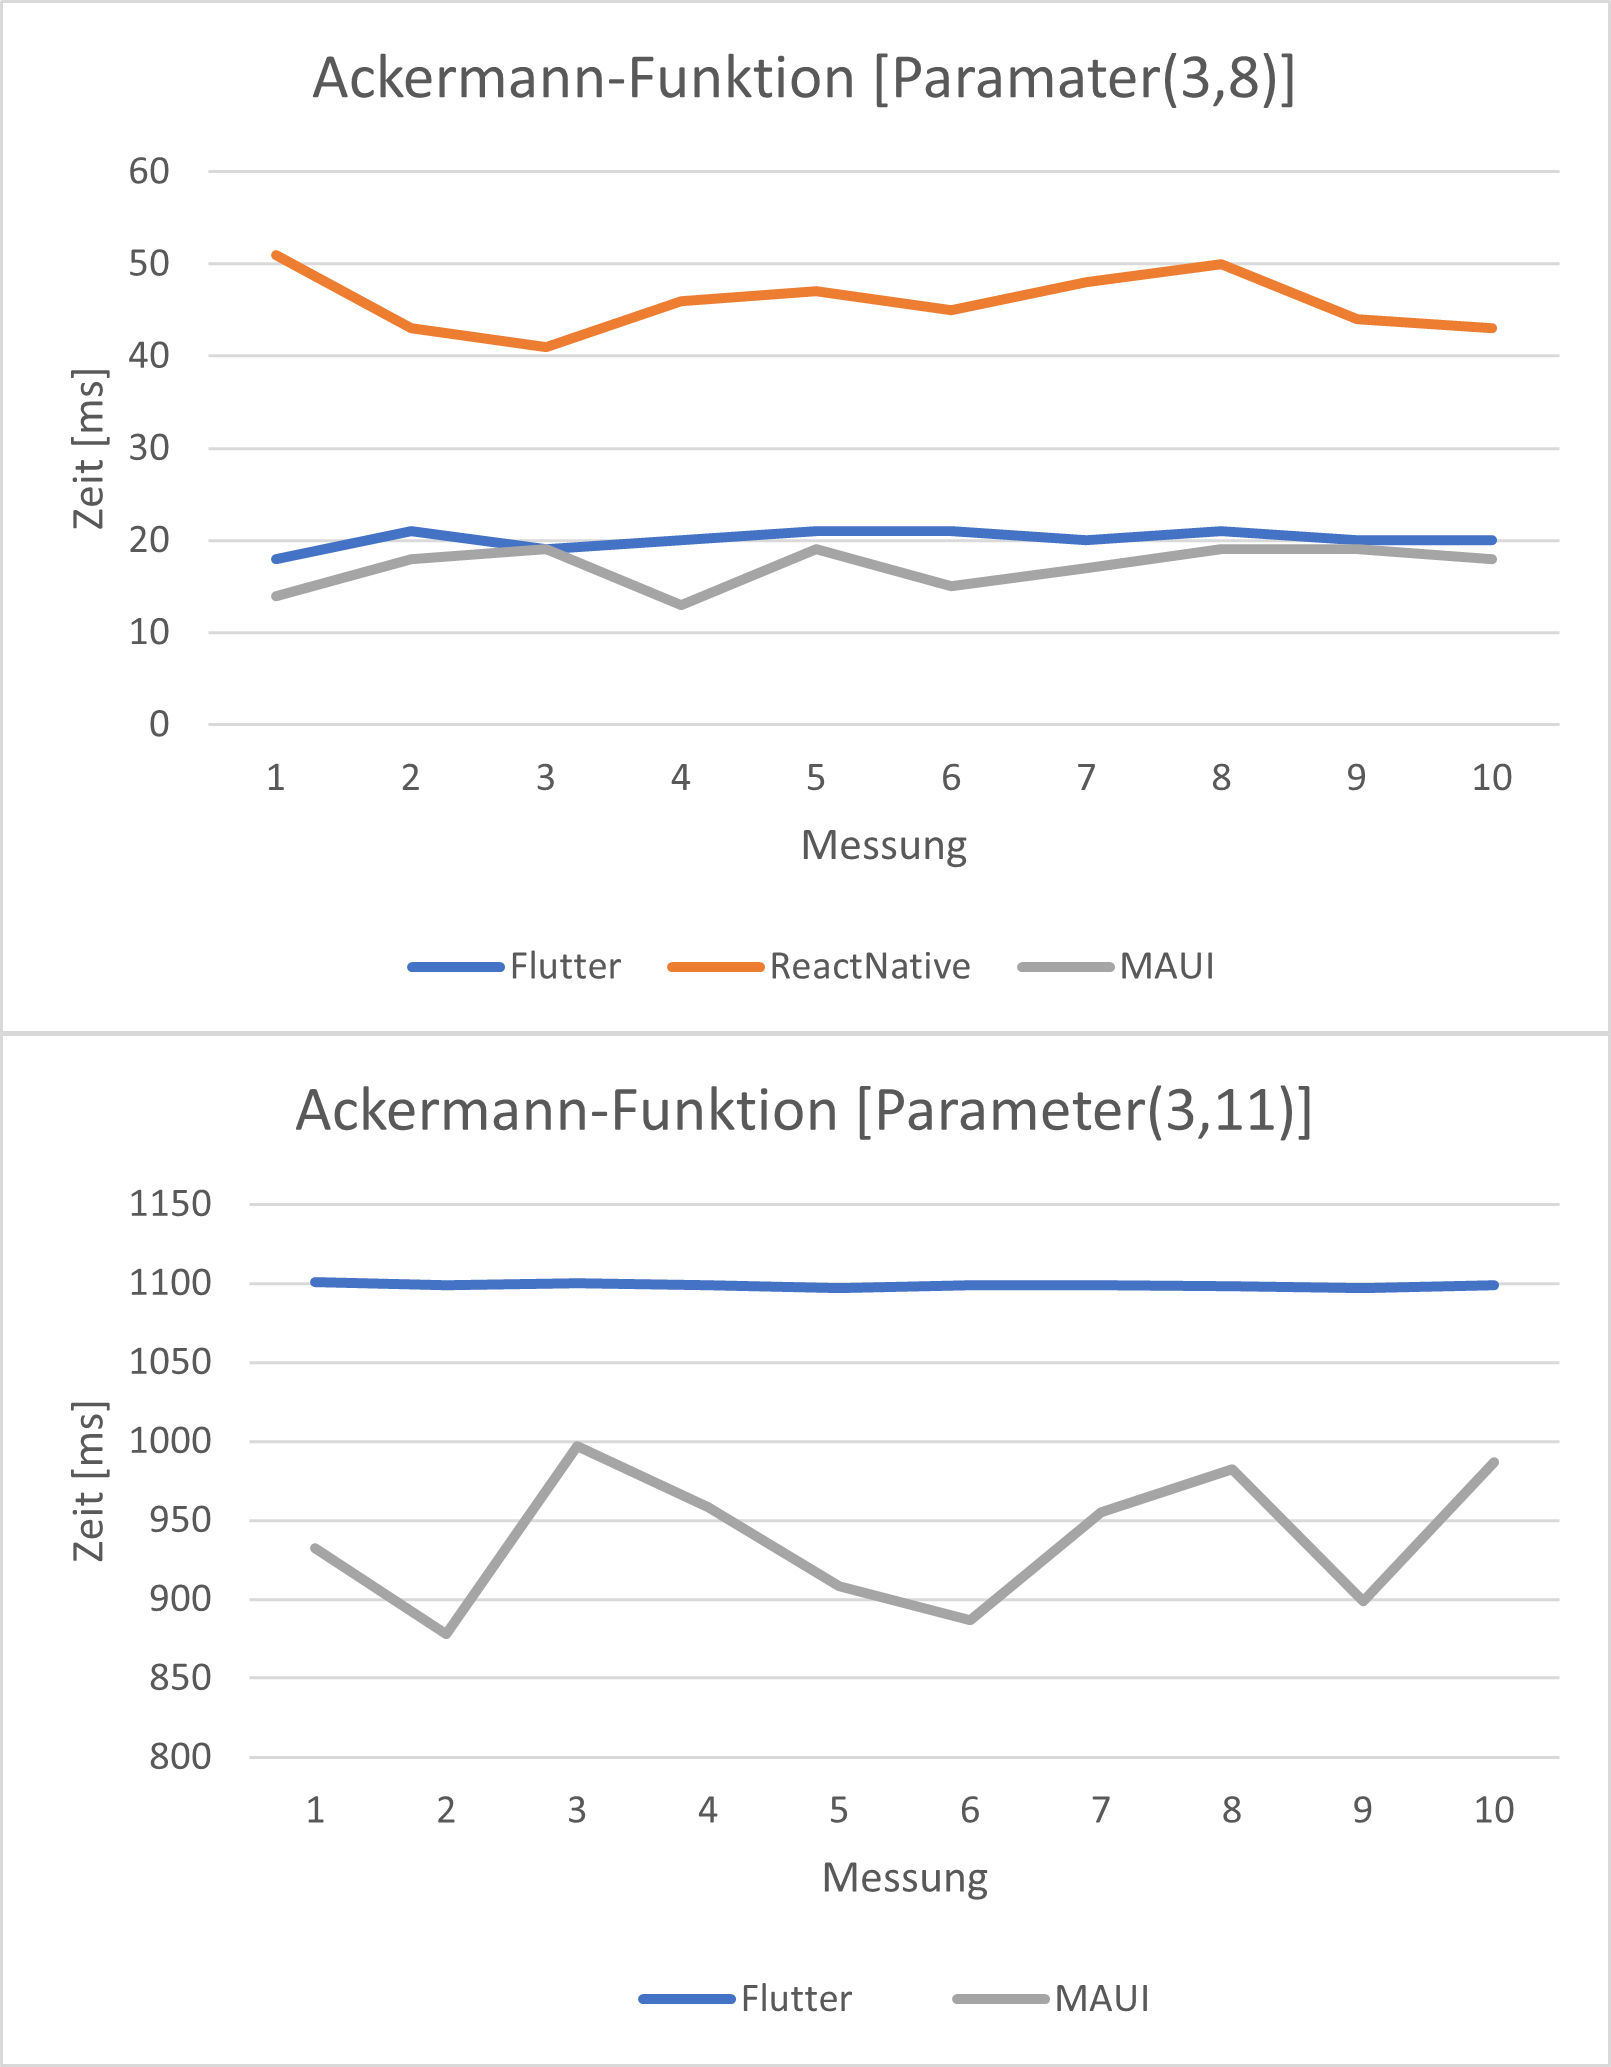
\includegraphics[width=0.75\linewidth]{images/ackermann}
	\caption{Analyse der Frameworks anhand der Ackermann-Funktion}
	\label{fig:ackerman}
\end{figure}
Bei der Durchführung der Messungen wurde festgestellt, dass Flutter und MAUI nur geringe Unterschiede bei der Ausführungszeit aufweisen. MAUI berechnet die Ackermann-Funktion bei beiden Varianten etwas schneller als Flutter. Konkret benötigt MAUI jeweils rund 15\% weniger Rechenzeit. Deutlich abgeschlagen ist in beiden Fällen das dritte Framework React Native. Bei den Parametern (n=3, m=8) benötigte es 2,5x länger als Flutter, um das Ergebnis der Ackermann-Funktion zu berechnen. Bei (n=3, m=12) konnte React Native kein Ergebnis errechnen und brach schon vorher mit einem StackOverflow-Fehler ab.

Bei der iterativen Potenzierung wurde mit der Basis 12 und dem Exponenten 9 gemessen. Die Messergebnisse sind in Abbildung \ref{fig:potenz} dargestellt.
\begin{figure}[ht]
	\centering
	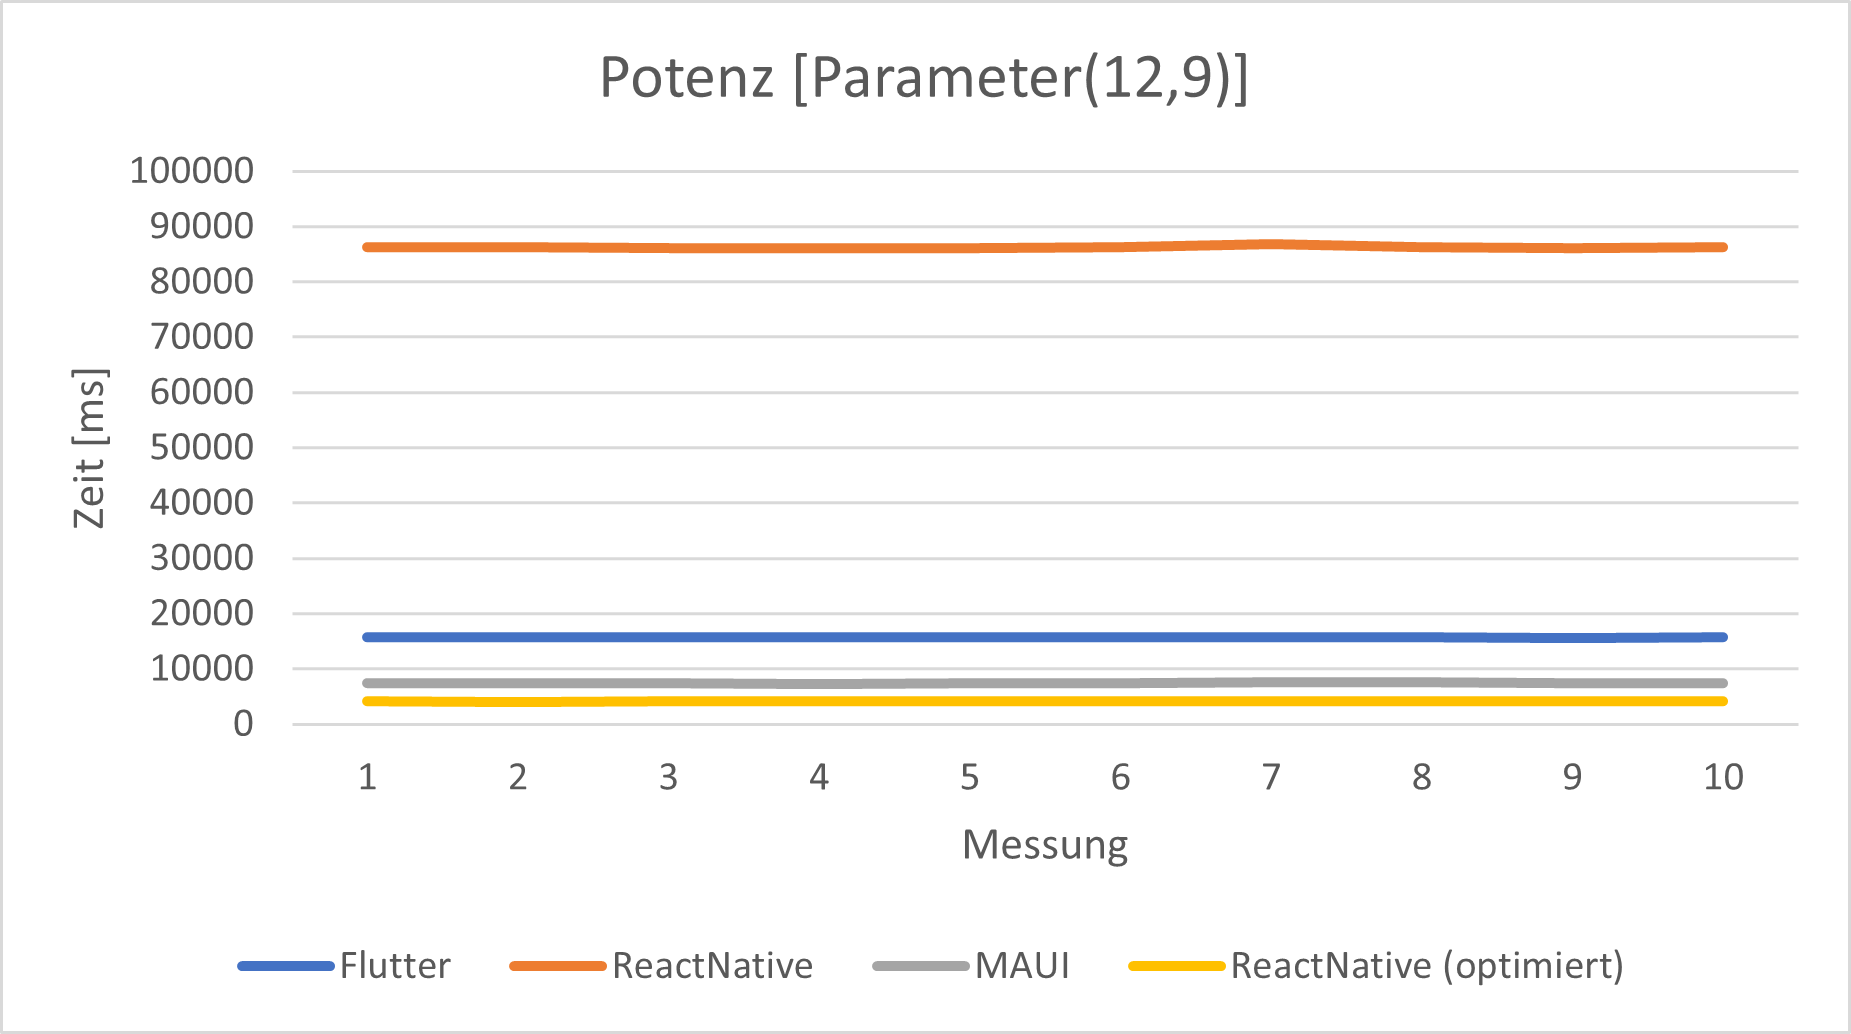
\includegraphics[width=0.8\linewidth]{images/potenz}
	\caption{Analyse der Frameworks anhand der Iterativen Potenzierung}
	\label{fig:potenz}
\end{figure}
Dabei ist derselbe Trend wie bei der Ackermann-Funktion erkennbar. MAUI hat erneut die höchste Performance und ist konkret 50\% schneller als Flutter. Außerdem ist React Native zeitlich erneut weit von den anderen Frameworks entfernt. Es benötigt rund 5,5x länger als Flutter zur Berechnung der Potenz. Durch Ausführung eines nativen Moduls war es möglich, ReactNative zu optimieren und ebenfalls eine hohe Performance zu erreichen.

Die Auslastung der CPU wurde bei einer rechenintensiven Berechnung über einen Zeitraum von 30 Sekunden gemessen. Die Messergebnisse sind in Abbildung \ref{fig:cpu} dargestellt. 
\begin{figure}[ht]
	\centering
	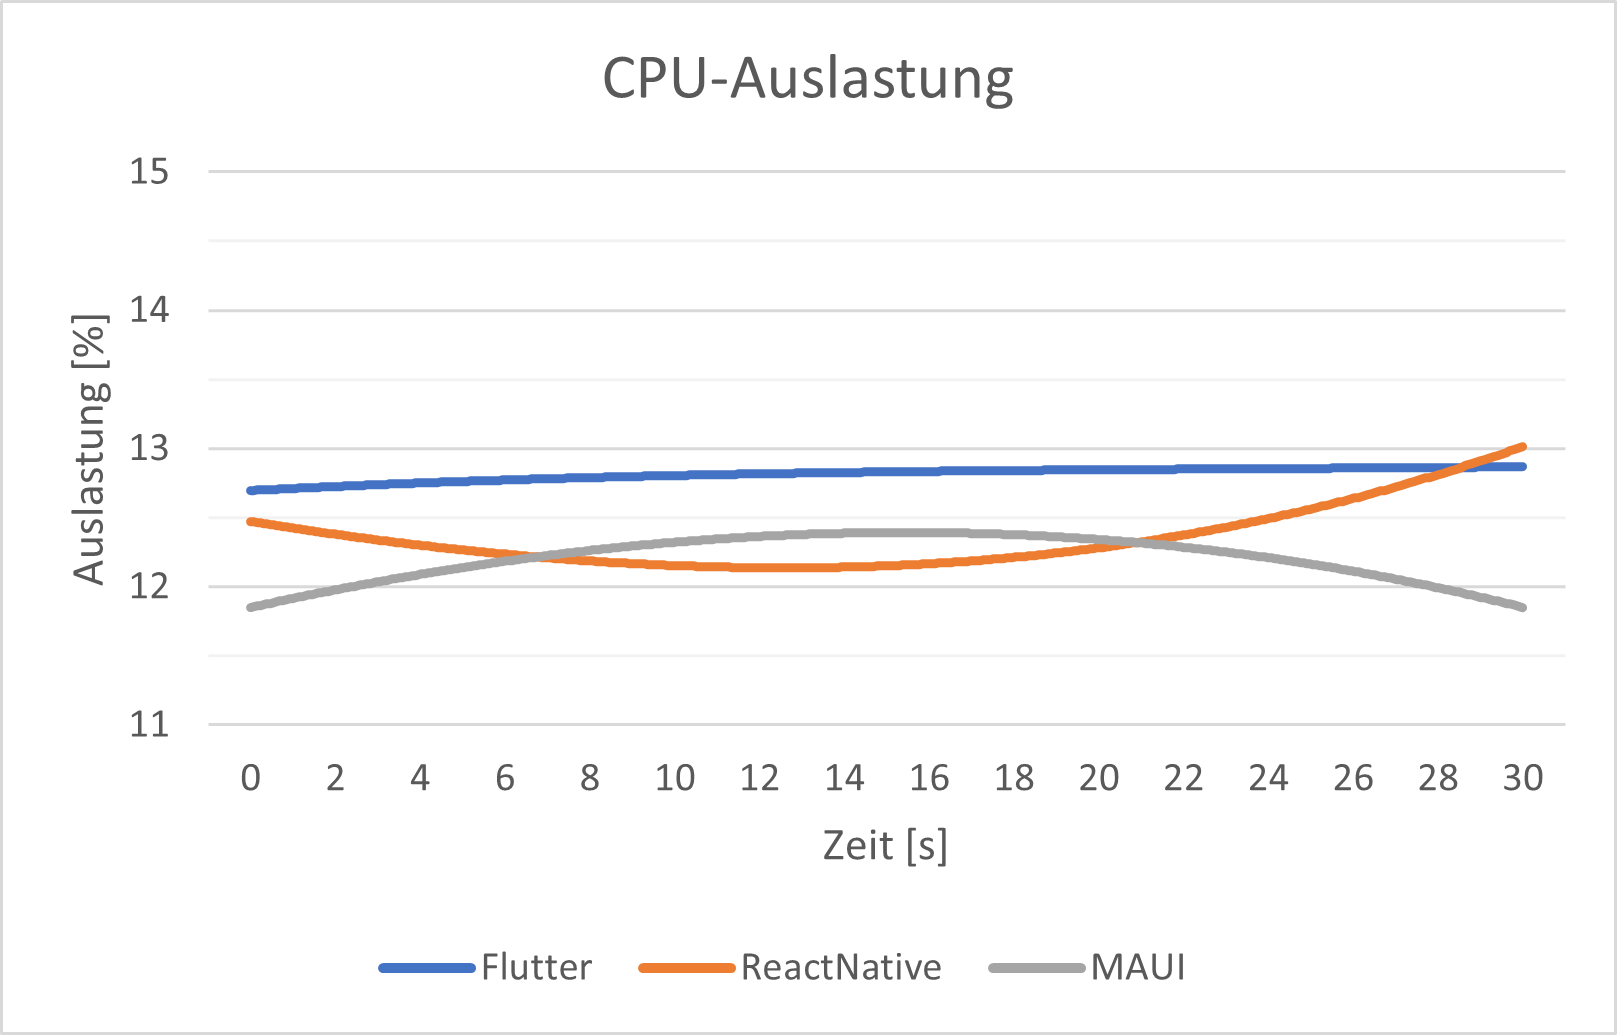
\includegraphics[width=0.8\linewidth]{images/cpu}
	\caption{CPU-Auslastung der Frameworks}
	\label{fig:cpu}
\end{figure}
Es ist sichtbar, dass alle Frameworks annähernd dieselben Auslastung generieren. Konkret lastet MAUI die CPU mit geringem Abstand am wenigsten aus, während Flutter tendenziell eine leicht höhere Auslastung herbeiführt.

\subsection{Bewertung der Frameworks} \label{sec:bewertung}
In diesem Abschnitt werden die Frameworks für die ermittelten Vergleichskriterien bewertet. Jedes Kriterium kann mit minimal 0 Punkten und maximal 5 Punkten bewertet werden. Dabei werden die ermittelten Eigenschaften der Frameworks aus der Literaturarbeit in Kapitel \ref{sec:frameworks} verwendet. Außerdem werden die Ergebnisse des Benchmarkings in Abschnitt \ref{sec:benchmarking} und die subjektiven Eindrücke bei der Erstellung der Prototypen miteinbezogen.

\subsubsection{Flutter}
Flutter erhält aufgrund der angegebenen Faktoren die folgenden Bewertungen.
\begin{description}
	\item[Plattformspezifische Funktionen (5/5)] Es ist ein einfacher Zugriff auf Sensoren des Endgeräts gegeben. Außerdem ist eine Möglichkeit zur eigenständigen Implementierung beim Zugriff auf plattformspezifische Schnittstellen vorhanden.
	\item[Performance (4/5)] Es liegt eine hohe Performance durch u.\,A. AOT-Kompilierung vor. Da Flutter laut Benchmarking minimal langsamer als MAUI ist, ist ein kleiner Punktabzug notwendig.
	\item[Benutzeroberfläche (4/5)] Flutter hat ein einzigartiges Design, da keine OEM-Widgets verwendet werden, sondern mit einer eigenen Renderengine gearbeitet wird. Es ist ein kleiner Punktabzug notwendig, da im Gegensatz zu den anderen Frameworks keine Gestaltung per CSS möglich ist.
	\item[Erste Schritte (2/5)] Es ist aufgrund der vergleichsweise aufwändigen Installation ein starker Punktabzug notwendig, da viele Abhängigkeiten zu anderen Programmen vorliegen. Die Einarbeitung in Dart kann Zeit benötigen, da der Aufbau der Anwendung teilweise nicht intuitiv ist.
	\item[Entwicklungsunterstützung (4/5)] Es ist eine Unterstützung für viele verschiedene IDEs inklusive Erweiterungen vorhanden. Durch Hot Reload wird eine schnelle Entwicklung ermöglicht. Es ist ein kleiner Punktabzug notwendig, da die Unterstützung beim Anlegen von Widgets besser sein könnte.
	\item[Dokumentation (5/5)] Die Dokumentation ist online und offline verfügbar und sehr umfangreich. Außerdem sind Videoanleitungen auf Youtube vorhanden.
	\item[Ökosystem (4/5)] Pakete können einfach über den Pub Package Manager eingebunden werden. Es ist eine umfangreiche Paketauswahl vorhanden. Ein kleiner Punktabzug ist notwendig, da kein vergleichbar großes Ökosystem wie z.\,B. bei .NET vorliegt.
	\item[Lebenszyklus \& öffentliches Interesse (5/5)] Flutter ist das meistverwendete, hybrides Framework im Jahr 2021 mit steigenden Tendenzen. Es ist sehr modern und noch am Beginn des Lebenszyklus, da der Release erst 2018 war.
\end{description}

\subsubsection{React Native}
React Native erhält aufgrund der angegebenen Faktoren die folgenden Bewertungen.
\begin{description}
	\item[Plattformspezifische Funktionen (5/5)] Es ist ein einfacher Zugriff auf Sensoren des Endgeräts gegeben. Außerdem sind Bibliotheken vorhanden, die Dateizugriffe übernehmen und einfach gestalten. Es gibt die Möglichkeit, über Android z.\,B. eigene Module zu implementieren.
	\item[Performance (2/5)] Es ist ein starker Punktabzug notwendig, da React Native eindeutig die geringste Performance der drei Frameworks hat. Die Optimierung durch native Module wiegt dies nicht auf.
	\item[Benutzeroberfläche (4/5)] Native Widgets des jeweiligen Systems werden verwendet. Das Design erfolgt über spezielles CSS, somit ist die Gestaltung sehr variabel. Ein kleiner Punktabzug ist notwendig, da keine eigenen, einzigartigen Widgets benutzt werden.
	\item[Erste Schritte (3/5)] Es ist ein kleiner Punktabzug notwendig, da die Installation etwas aufwändiger ist. Nach der Installation genügen allerdings einfache Befehle zur Erstellung von Apps.
	\item[Entwicklungsunterstützung (4/5)] Viele verschiedene IDEs inklusive Erweiterungen werden unterstütz. React Native ist z.\,B. in der IDE Webstorm von JetBrains bereits bei Installation vorhanden. Es ist ein kleiner Punktabzug notwendig, da die Unterstützung beim Anlegen von Widgets besser sein könnte.
	\item[Dokumentation (5/5)] Die Dokumentation ist online umfangreich verfügbar. Außerdem sind zahlreiche Bücher erhältlich.
	\item[Ökosystem (4/5)] Über NPM können Module einfach per Terminal hinzugefügt werden. Eine umfangreiche Paketauswahl ist ebenfalls vorhanden. Ein kleiner Punktabzug ist notwendig, da kein vergleichbar großes Ökosystem wie z.\,B. bei .NET vorliegt.
	\item[Lebenszyklus \& öffentliches Interesse (5/5)] React Native wird für viele bekannte Apps verwendet und durch Meta weiterentwickelt. Das Framework ist ausgereift, da es bereits seit 2015 auf dem Markt ist.
\end{description}

\subsubsection{MAUI}
MAUI erhält aufgrund der angegebenen Faktoren die folgenden Bewertungen.
\begin{description}
	\item[Plattformspezifische Funktionen (4/5)] Der Zugriff auf Sensoren des Endgeräts ist durch Pakete gegeben. Eine Möglichkeit zur eigenständigen Implementierung in C\# beim Zugriff auf plattformspezifische Schnittstellen ist vorhanden. Es ist ein kleiner Punktabzug notwendig, da der Zugriff auf Sensoren aufwändiger als in den anderen Frameworks ist.
	\item[Performance (5/5)] MAUI hat u.\,A. durch die AOT-Kompilierung eine sehr hohe Performance. Es ist minimal schneller als Flutter und deutlich schneller als React Native.
	\item[Benutzeroberfläche (4/5)] Die Gestaltung der Oberfläche erfolgt über HTML und CSS. Bereits erstellte Webanwendungen können wiederverwendet werden. Ein kleiner Punktabzug ist notwendig, da keine eigenen, einzigartigen Widgets benutzt werden.
	\item[Erste Schritte (5/5)] Die Installation und Einrichtung ist sehr einfach, da Visual Studio den Großteil der Arbeit abnimmt und Abhängigkeiten nachinstalliert. Der Aufbau der Anwendungen ist intuitiv und orientiert sich an anderen Microsoft-Produkten.
	\item[Entwicklungsunterstützung (4/5)] Unterstützung für viele verschiedene IDEs ist vorhanden. Die Hot Reload-Funktion ermöglicht eine schnelle Entwicklung und funktioniert zuverlässig. Der Android Emlator ist direkt in Visual Studio integriert. Ein kleiner Punktabzug ist notwendig, da die Unterstützung beim Anlegen von Widgets besser sein könnte.
	\item[Dokumentation (4/5)] Die Dokumentation ist online umfangreich verfügbar. Außerdem sind Videoanleitungen und Lernplattformen vorhanden. Es gibt einen kleinen Punktabzug, da Verwechslungsgefahr zwischen klassischem MAUI (via XAML) und MAUI Blazor besteht.
	\item[Ökosystem (5/5)] Der NuGet Package Manager kann zum Einbinden von Paketen entweder im Terminal oder auf einer grafischen Oberfläche verwendet werden. Das .NET-Ökosystem ist sehr umfangreich und es werden viele Anwendungsbereiche unterstützt.
	\item[Lebenszyklus \& öffentliches Interesse (3/5)] MAUI ist ein sehr junges Framework mit großem Interesse im .NET-Umfeld. Es steht am Beginn des Lebenszyklus, da der Release erst 2022 war. Es ist ein kleiner Punktabzug notwendig, da noch kleinere Fehler bzw. \glqq Kinderkrankheiten\grqq\:im Framework vorhanden sind.
\end{description}


\subsection{Vergleich und Ergebnisse}
% (2 Seiten)
Im Folgenden werden die in Abschnitt \ref{sec:bewertung} ermittelten Bewertungen der Frameworks unter Berücksichtigung der in Abschnitt \ref{sec:gewichtung} definierten Gewichtungen der Vergleichskriterien je Anwendungsgebiet miteinander verglichen.

\subsubsection{Formularlastige Anwendung}

\begin{figure}[ht]
	\centering
	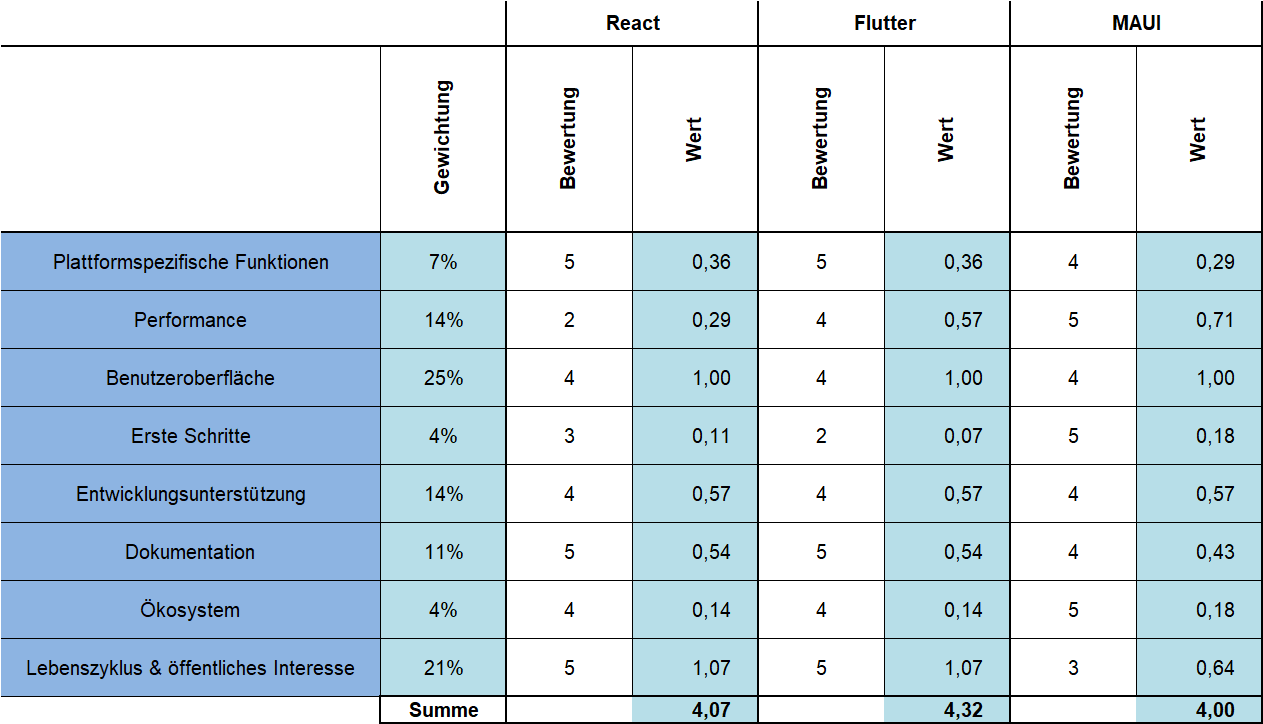
\includegraphics[width=0.8\linewidth]{images/AnalyseFormularlastig.png}
	\caption{Bewertung für formularlastige Anwendungen}
	\label{fig:analFormular}
\end{figure}

Im Anwendungsgebiet der formularlastigen Anwendungen setzt sich Flutter mit einer Gesamtbewertung von 4,32 gegen React Native mit 4,07 und MAUI mit 4,00 durch. Alle Frameworks erreichen eine Wertung von größer oder gleich 4 Punkten von den maximal erreichbaren 5 Punkten. In dem für dieses Anwendungsgebiet am höchsten gewichteten Vergleichskriterium schneiden alle Frameworks gleich gut ab. Das Bewertungsschema der einzelnen Vergleichskriterien je Anwendungsgebiet und Framework, sowie die Gesamtbewertung eines jeden Frameworks ist in Abbildung \ref{fig:analFormular} dargestellt.


\subsubsection{Rechenintensive Anwendung}

\begin{figure}[ht]
	\centering
	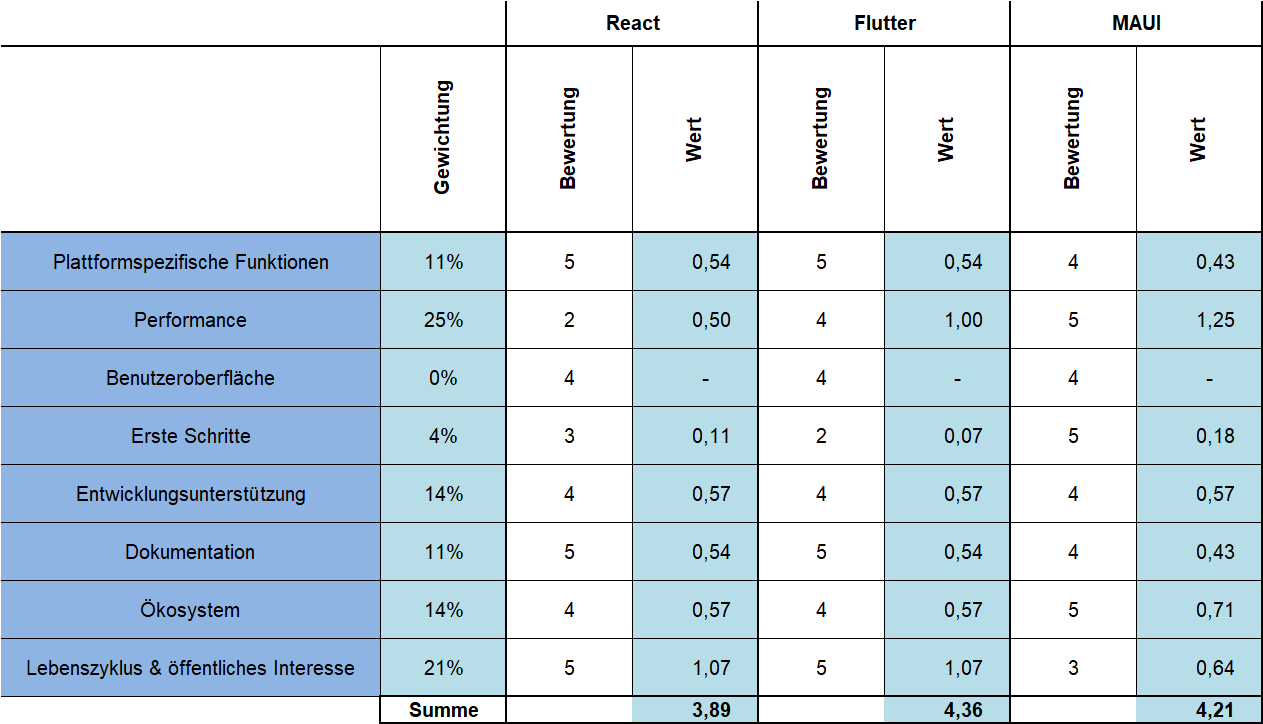
\includegraphics[width=0.8\linewidth]{images/AnalyseRechenintensiv.png}
	\caption{Bewertung für rechenintensive Anwendungen}
	\label{fig:analRechen}
\end{figure}

Im Anwendungsgebiet der rechenintensiven Anwendungen setzt sich Flutter mit einer Gesamtbewertung von 4,36 gegen MAUI mit 4,21 und React Native mit 3,89 durch. Lediglich Flutter und MAUI erreichen eine Wertung von größer oder gleich 4 Punkten von den maximal erreichbaren 5 Punkten. In dem für dieses Anwendungsgebiet am höchsten gewichteten Vergleichskriterium schneidet MAUI am besten ab, dennoch erreicht Flutter eine höhere Gesamtwertung. React Native schneidet bei diesem Vergleichskriterium am schlechtesten ab. Das Bewertungsschema der einzelnen Vergleichskriterien je Anwendungsgebiet und Framework, sowie die Gesamtbewertung eines jeden Frameworks ist in Abbildung \ref{fig:analRechen} dargestellt.

\subsubsection{Sensorlastige Anwendung}

\begin{figure}[ht]
	\centering
	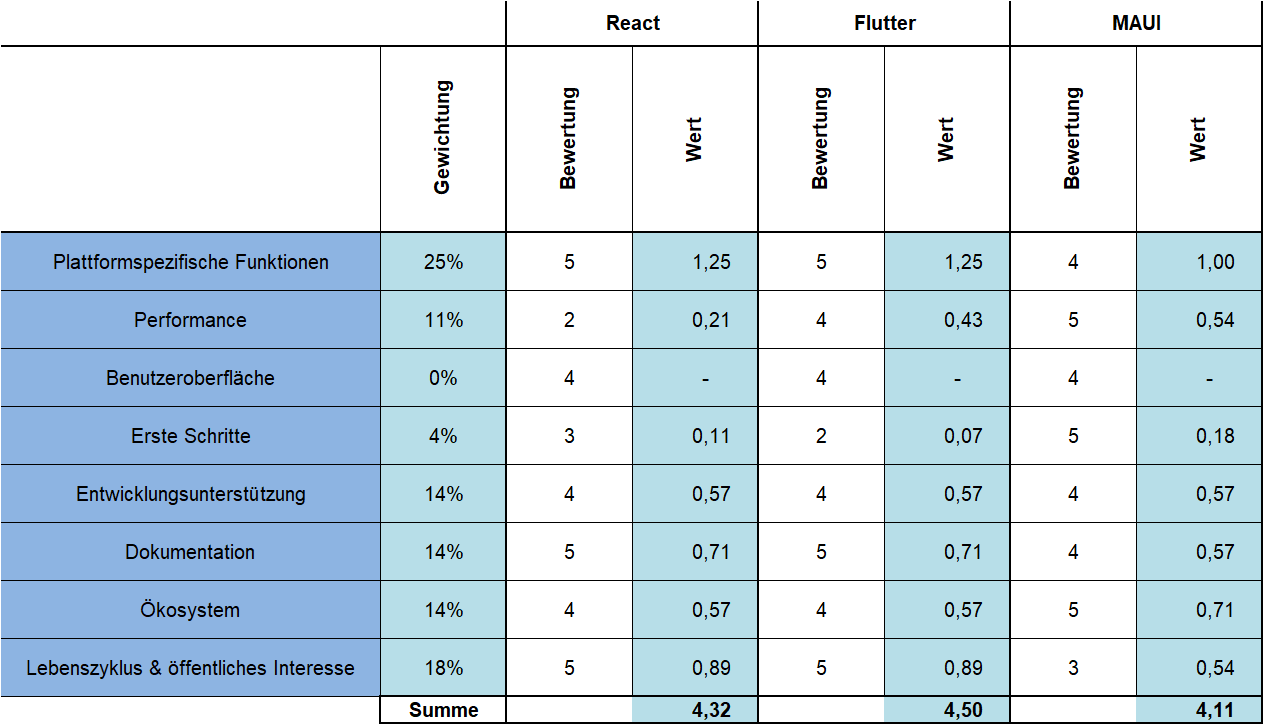
\includegraphics[width=0.8\linewidth]{images/AnalyseSensorlastig.png}
	\caption{Bewertung für sensorlastige Anwendungen}
	\label{fig:analSensor}
\end{figure}

Im Anwendungsgebiet der sensorlastigen Anwendungen setzt sich Flutter mit einer Gesamtbewertung von 4,50 gegen React Native mit 4,32 und MAUI mit 4,11 durch. Alle Frameworks erreichen eine Wertung von größer oder gleich 4 Punkten von den maximal erreichbaren 5 Punkten. In dem für dieses Anwendungsgebiet am höchsten gewichteten Vergleichskriterium erhalten Flutter und React Native die maximal erreichbare Punktzahl. MAUI schneidet beim bei diesem Vergleichskriterium etwas schlechter ab. Das Bewertungsschema der einzelnen Vergleichskriterien je Anwendungsgebiet und Framework, sowie die Gesamtbewertung eines jeden Frameworks ist in Abbildung \ref{fig:analSensor} dargestellt.

\subsubsection{Ergebnis}
In Abbildung \ref{fig:ergebnis} ist das Ergebnis des Vergleichs übersichtlich zusammengefasst. Es ist erkennbar, dass Flutter insgesamt die beste Bewertung erreicht hat. Dahinter folgen mit einigem Abstand MAUI und ReactNative.

\begin{figure}[ht]
	\centering
	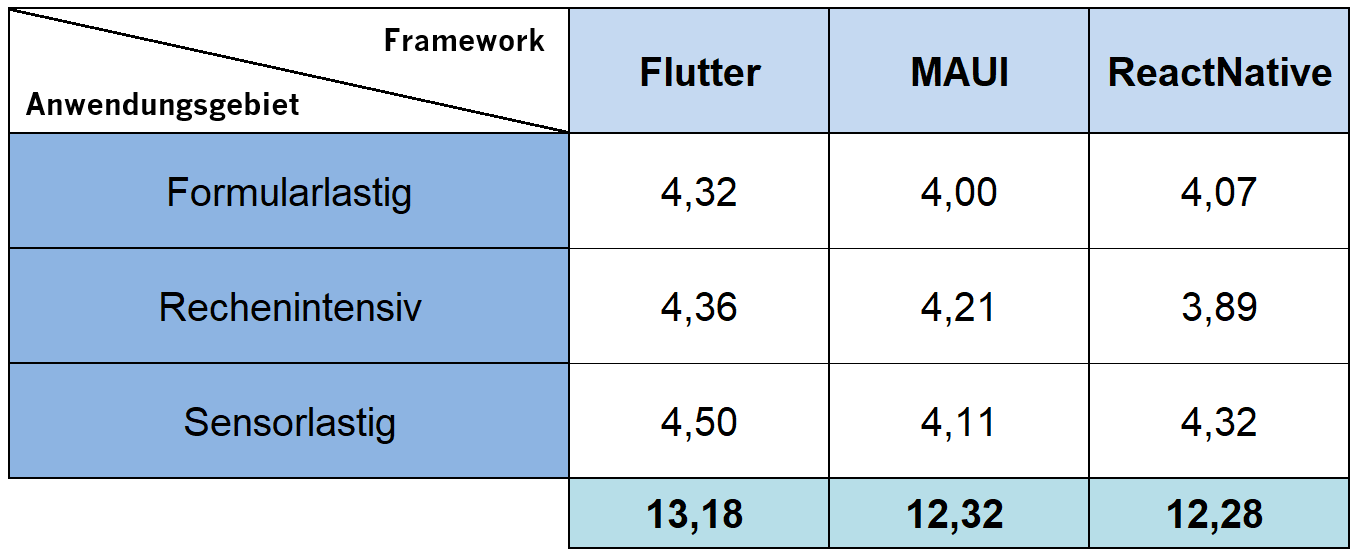
\includegraphics[width=0.8\linewidth]{images/ergebnis.png}
	\caption{Übersicht über Punktzahlen je Framework und Anwendungsgebiet}
	\label{fig:ergebnis}
\end{figure}

\clearpage

\section{Fazit}
% ca. 1 Seite
Alle drei Frameworks erleichtern die Entwicklung von mobilen Applikationen, indem der Kern der Applikation nur einmal entwickelt werden muss. So kann viel Zeit gespart werden, die sonst in die Entwicklung separater Anwendungen in unterschiedlichen Programmiersprachen für jedes einzelne Betriebssystem investiert werden müsste. Bei allen getesteten Frameworks wird die Erstellung einer Web-App, einer Android-App und einer iOS-App unterstützt. Außerdem ist abhängig vom individuellen Framework die Entwicklung für weitere Systeme möglich. So kann man z.\,B. mit Maui und React Native Windows-Store-Apps erstellen, während Flutter die Erstellung von Windows Executables ermöglicht.

Alle Frameworks überzeugen durch eine gute, ausführliche Online-Dokumentation. Bei Flutter stellte sich die Einrichtung jedoch als etwas komplizierter heraus, da viele Abhängigkeiten zu anderen Programmen bestehen. Außerdem erlauben alle Frameworks eine große Vielfalt an Gestaltungsmöglichkeiten, da z.\,B. die Gestaltung durch eine eingeschränkte Form von CSS möglich ist. Sowohl React Native als auch Maui bringen zudem den Vorteil mit sich, dass der Code von bereits existierenden Web-Apps übernommen werden kann. Da hinter allen Frameworks namhafte Firmen wie Microsoft, Google und Meta stehen, kann man davon ausgehen, dass die Frameworks auch in Zukunft weiterentwickelt werden und weiter unterstützt werden.

Bei der Durchführung des Benchmarkings konnte ermittelt werden, dass die Prototypen der Frameworks Flutter und Maui sehr performant sind. Das Framework React Native ist hingegen deutlich weniger performant. Die CPU-Auslastung ist bei allen Frameworks nahezu identisch.

Mit einer formularlastigen Anwendung, einer sensorlastigen Anwendung und einer rechenintensiven Anwendung wurden drei Anwendungsgebiete definiert. Durch die Ermittlung von Vergleichskriterien, einer individuellen Gewichtung je Anwendungsgebiet und einer anschließenden Bewertung konnten je Framework und Anwendungsgebiet Punktzahlen berechnet werden. Dabei konnte sich Flutter in jedem Anwendungsgebiet vor MAUI und React Native durchsetzen. Das abschließende Ergebnis des Vergleichs ist in Abbildung \ref{fig:ergebnis} dargestellt. Es ist ersichtlich, dass Flutter insgesamt die beste Bewertung erreicht hat. Auf dem zweiten Platz befindet sich MAUI, auf dem dritten Platz folgt React Native.

\clearpage

%%% Angabe der .bib-Datei (ohne Endung) / State .bib file (for BibTeX usage)
\printbibliography %\printbibliography if you use biblatex/Biber
\end{document}